\PassOptionsToPackage{hidelinks}{hyperref}

\documentclass[doc,biblatex]{apa7}

\usepackage{amsmath}
\usepackage{mathspec}
\usepackage{xeCJK} % for Chinese characters

% temp for revision %%%%%%%%%%%%%%%%%%%%%%%%%%%%
\usepackage{xcolor}
\newcommand\newmaterial[1]{\textcolor{blue}{#1}}
%%%%%%%%%%%%%%%%%%%%%%%%%%%%%%%%%%%%%%%%%%%%%%%%

\DeclareLanguageMapping{american}{american-apa}
\addbibresource{references.bib}

\captionsetup[figure]{textfont=rm,font=small,labelfont=bf}
\setallmainfonts{Times New Roman}
\setmainfont{Times New Roman}

\title{Why do languages tolerate heterography? An experimental investigation into the emergence of informative orthography}

\shorttitle{Why do languages tolerate heterography?}

\authorsnames{Anonymous}

\authorsaffiliations{{Anonymous}}

\abstract{It is widely acknowledged that opaque orthographies place additional demands on learning, often requiring many years to fully acquire. It is less widely recognized, however, that such opacity may offer certain benefits in the context of reading. For example, heterographic homophones such as <knight> and <night> (words that sound the same but which are spelled differently) impose additional costs in learning but reduce ambiguity in reading. Here, we consider the possibility that---left to evolve freely---writing systems will sometimes choose to forego some simplicity for the sake of informativeness when there is functional pressure to do so. We investigate this hypothesis by simulating the evolution of orthography as it is transmitted from one generation to the next, both with and without a communicative pressure for ambiguity avoidance. In addition, we consider two mechanisms by which informative heterography might be selected for: \textit{differentiation}, in which new spellings are created to differentiate meaning (e.g., <lite> vs.~<light>), and \textit{conservation}, in which heterography arises as a byproduct of sound change (e.g., <meat> vs.~<meet>). Under pressure from learning alone, orthographic systems become transparent, but when combined with communicative pressure, they tend to favor some additional informativeness. Nevertheless, our findings also suggest that, in the long term, simpler, transparent spellings may be preferred in the absence of top-down explicit teaching.}

\keywords{communication; iterated learning; language evolution; orthography; reading; writing}

\begin{document}

\maketitle

\noindent
Writing systems, particularly those employing alphabetic scripts, are commonly regarded as providing a visual representation of speech, with letters or chunks of letters corresponding to distinct sounds. However, it is also well understood that writing systems diverge from their spoken counterparts in important ways \parencite{Biber:1988, Bolinger:1946, Coulmas:1991}. The insertion of spacing between words, for example, is almost ubiquitous across alphabetic writing systems, even though no such spacing exists between words in speech \parencite{Parkes:1992, Saenger:1997}. It seems likely that graphic innovations such as these exist because they confer some benefit that is not required in the spoken modality \parencite{Rastle:2019}. In the case of spacing, for example, the separation of words into discrete chunks presumably aids in the targeting and extraction of visuo-linguistic information---constraints that do not exist in the auditory modality. In principle, the same may be true of spelling: Words may be spelled in ways that diverge from the spoken language because such divergence confers some benefit in reading \parencite{Ulicheva:2020}.

One potential case of such functional divergence is heterographic homophony---words that sound alike but which are written differently (e.g., <meat> and <meet> for /miːt/). Heterographic spellings such as these may serve a valuable function in reading. For example, an English speaker faced with a spoken sentence beginning /ðɛr.../ will have high uncertainty about what word---or even what sentence structure---is likely to come next: a noun, as in /ðɛr~kat/, a form of the verb \textit{to~be}, as in /ðɛr~ɪz/, or the progressive form of a verb, as in /ðɛr~gəʊɪŋ/. In writing, by contrast, this uncertainty is greatly reduced; the spellings <their>, <there>, and <they're> differentiate these cases, giving the reader a headstart on processing the upcoming syntactic structure and semantic content. Heterographic homophony is also common below the word level, since many orthographies forego the phonological principle in favor of the morphological principle in the spelling of affixes \parencite{Sandra:2024}. The English suffixes \textit{-er} (denoting the comparative form of an adjective; e.g., \textit{nicer}) and \textit{-or} (denoting the performer of an action; e.g., \textit{actor}) are homophonous in speech (/ər/), but their spellings differentiate these meanings in writing. Of course, English orthography is suboptimal here in~that \textit{-er} may also indicate agentive status (e.g., \textit{builder}); nevertheless, statistical patterns such as these hold across a variety of English affixes \parencite{Berg:2017} and it has been shown that readers are sensitive to and make use of such cues in reading \parencite{Ulicheva:2020}. \newmaterial{Heterography might be especially important given the differing constraints of the written modality, including the lack of other cues to meaning, such as stress, context, and body language, and the inability for reader and writer to engage in immediate feedback and repair. Furthermore, written language has richer vocabulary and more complex syntax than spoken language \parencite{Biber:1988, Korochkina:2024, Nation:2022}, placing different pressures on ambiguity resolution.}

\newmaterial{Heterography is particularly notable in English, but it is also a feature of many other languages and writing systems. French is similar to English in having a large number of heterographic homophones: \textit{cent} (\textit{hundred}), \textit{sang} (\textit{blood}), \textit{sans} (\textit{without}), and \textit{sens} (\textit{feel}), for example, are all pronounced /sɑ̃/ (although their pronunciations will sometimes be distinguished through liaison). In Danish, the words \textit{hver} (\textit{every}), \textit{vejr} (\textit{weather}), \textit{vær} (\textit{be}), and \textit{værd} (\textit{worth}) are all pronounced /vεˀɐ̯/. In Vietnamese, the graphemes <d>, <gi>, and <r> are homophonous, resulting in sets like \textit{dao} (\textit{knife}), \textit{giao} (\textit{delivery}), and \textit{rao} (\textit{advertise}), all pronounced /zāw/. In some cases, features of an orthography designed for other purposes can inadvertently result in homophone disambiguation: Noun capitalization in German contrasts \textit{Wagen} (\textit{car}) and \textit{wagen} (\textit{to dare}), both pronounced /vaːɡṇ/; eclipsis marking in Irish contrasts \textit{bpáistí} (\textit{children}) and \textit{báistí} (\textit{rain}), both pronounced /bɑʃti/; and the morphological principle of Russian orthography contrasts \textit{приступить} (\textit{to start}) and \textit{преступить} (\textit{to transgress}), both pronounced /pristupʲitʲ/. Even in the most transparent of orthographies it is possible to find some instances of heterography: In Italian, the residual~\textsc{h} inherited from Latin contrasts \textit{hanno} (\textit{have}) and \textit{anno} (\textit{year}), both pronounced /anno/, while the grave accent is sometimes used to distinguish common homophonous words, such as \textit{la} (\textit{the}) and \textit{là} (\textit{there}).}

\newmaterial{Perhaps the most elaborate example of how a writing system can deal with homophony head-on is the Chinese orthography. The Chinese spoken languages are rich in homophones, making heterographic spellings---and therefore a logographic writing system---particularly useful \parencite{Frost:2012}. In Mandarin Chinese, the words 糖 (\textit{sugar}), 塘 (\textit{embankment}), 溏 (\textit{pond}), and 搪 (\textit{to block}) are homophonous in speech but heterographic in writing---the phonetic radical on the right (<唐>, /táŋ/) represents the spoken syllable, while the semantic radicals on the left differentiate the meanings \parencite[p.~101]{Coulmas:1991}. In addition, 唐 itself is a surname/dynasty (\textit{Tang}), and another unrelated word 堂 (\textit{hall}) is also pronounced /táŋ/, yielding at~least six ways to write the same sound depending on the meaning. This property allows the written form of Chinese to convey more information about meaning---to be more \textit{informative}---than its spoken counterpart.}

Despite the benefits that heterography may provide in reading, it comes with two main costs. Firstly, by definition, heterography implies that a single sound can be spelled multiple ways. In English, the heterographic spellings <meat> and <meet> imply that /i/ can be spelled <ea> or <ee>. Readers are therefore required to learn alternate spellings for a single sound, \newmaterial{resulting in longer learning periods and more difficult decoding \parencite{Reis:2020, Seymour:2003, Spencer:2003, Taylor:2011, Zhao:2018}}. Secondly, the arbitrary mapping between heterographic forms and meaning must also be learned. From the point of view of a modern English speaker, there is no intrinsic reason why \textit{meat} is spelled <ea> and \textit{meet} is spelled <ee>. Nevertheless, these arbitrary spelling distinctions must be learned if they are to be useful, and they presumably place an additional burden on reading and---perhaps even more-so---on writing \parencite{Frith:1979, Shankweiler:1992}.

\newmaterial{In this paper, we consider the possibility that---left to evolve freely---writing systems will sometimes choose to forego some simplicity for the sake of informativeness.} A simple spelling system would be one that is easy to learn, use, and process; for example, by being transparent with respect to phonology. An informative spelling system, on the other hand, would be one that precisely conveys meaning. This idea of a tradeoff between simplicity and informativeness in the writing system has long been noted \parencite[e.g.,][]{Coulmas:1991}, and such a tradeoff has also been discussed within the study of language more broadly \parencite[e.g.,][]{Gabelentz:1891, Zipf:1949, Martinet:1952, Rosch:1978}. Recent typological \parencite[e.g.,][]{Kemp:2018} and experimental \parencite[e.g.,][]{Kirby:2015} studies have also subjected these ideas to empirical investigation in various domains. Of particular note here is the finding that complex, systematic structure emerges under concurrent pressures to be both simple and informative, a point we return to shortly.

First, however, it is useful to consider the mechanisms by which selection could occur if it is indeed the case that heterography emerges for functional reasons. \textcite[pp.~325--326]{Berg:2021} outline two models of how a word might enter a state of heterography. The first model, \textit{the differentiation model} (Fig.~\ref{models_of_heterography}A), explains heterography through the creation of new orthographic forms. For example, the spelling <lite> for the word \textit{light} is frequently used in food products to mean light-in-calorific-weight; in British English, the spelling <cheque> (\newmaterial{perhaps influenced by French \textit{chèque}}) differentiates the bank draft from other meanings of the word \textit{check}; and the word \textit{byte} was a deliberate respelling of \textit{bite} to avoid accidental mutation into the closely related term \textit{bit} \parencite{Buchholz:1977}. Many monosyllabic words that are homophonous with common function words also tend to adopt alternate spellings, often by adding <e> or by doubling the final consonant: \textit{be}--\textit{bee}, \textit{but}--\textit{butt}, \textit{by}--\textit{bye}--\textit{buy}, \textit{for}--\textit{fore}--\textit{four}, \textit{in}--\textit{inn}, \textit{or}--\textit{oar}--\textit{ore}, \textit{so}--\textit{sew}, \textit{to}--\textit{too}--\textit{two}, \textit{we}--\textit{wee}. Differentiation is also common in surnames---\textit{Clarke}, \textit{Greene}, \textit{Wilde}; \textit{Carr}, \textit{Hogg}, \textit{Mann}---and trade names---\textit{Blu Tack}, \textit{Froot Loops}, \textit{Wite-Out} \parencite[§~6]{Carney:1994}. One important way in which differentiation can occur---especially in a language like English that has historically contained a lot of spelling variation \parencite{Nevalainen:2012, Stenroos:2016}---is by the conditioning of variant spellings on meaning; pairs like \textit{discreet}--\textit{discrete}, \textit{flour}--\textit{flower}, and \textit{plain}--\textit{plane}, which were once variant spellings of the same word, have taken on distinct meanings over time \parencite[§~5.4]{Carney:1994}. \textcite[p.~58]{Berg:2017} have referred to this as the ``functionalization of leftovers'': The spelling variants that survive are those that ``can find distributional or functional niches.''

	\begin{figure}
	\makebox[\textwidth][c]{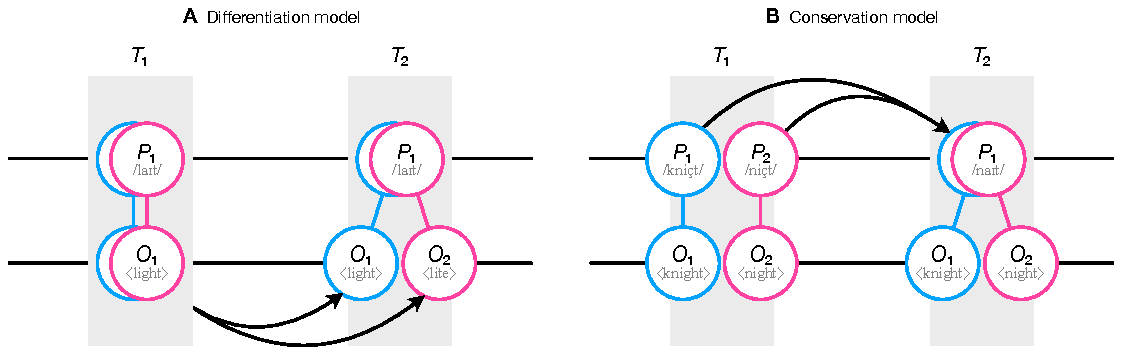
\includegraphics[scale=0.8]{figs/models_of_heterography.pdf}}
	\vspace*{2pt}
	\caption{Two models of heterography. \textbf{A} In the differentiation model, two meanings are, at time $T_1$, expressed by a single phonetic form $P_1$ and a single orthographic form $O_1$; however, by time $T_2$, two orthographic forms have emerged to differentiate the meanings in writing. \textbf{B} In the conservation model, the two distinct phonetic forms that existed at time $T_1$ have become homophonous by time $T_2$, but the two corresponding orthographic forms have been conserved, resulting in the same state of heterography as in the differentiation model. Adapted from \textcite[pp.~325--326]{Berg:2021} with permission.}
	\label{models_of_heterography}
	\end{figure}

The second model, \textit{the conservation model} (Fig.~\ref{models_of_heterography}B), explains heterographic homophones as the historical residue of sound change: Two spoken forms merge and become homophonous, but the original spellings are conserved in the orthography. For example, the \textit{meat}--\textit{meet} merger that occurred during the Great Vowel Shift ultimately resulted in Middle English /ɛː/ (spelled <ea>) and /eː/ (spelled <ee>) being pronounced /iː/ in Early Modern English \parencite{Lass:2000}, but the spellings were never changed accordingly, thus giving rise to a set of heterographic homophones that persist in present-day English \parencite[pp.~140--141]{Wells:1982}: \textit{heal}--\textit{heel}, \textit{leak}--\textit{leek}, \textit{meat}--\textit{meet}, \textit{read}--\textit{reed}, \textit{sea}--\textit{see}, \textit{team}--\textit{teem}, \textit{weak}--\textit{week}. The same is true of the \textit{pain}--\textit{pane} merger \parencite[pp.~141--142]{Wells:1982}: \textit{maid}--\textit{made}, \textit{main}--\textit{mane}, \textit{pain}--\textit{pane}, \textit{raise}--\textit{raze}, \textit{sail}--\textit{sale}, \textit{vain}--\textit{vane}. Sound changes involving consonants have also resulted in (or contributed to) pairs of words entering a state of heterography, such as the reduction of /kn/ into /n/ (e.g., \textit{knight}--\textit{night}, \textit{know}--\textit{no}, \textit{knot}--\textit{not}), the loss of /ç/ (e.g., \textit{eight}--\textit{ate}, \textit{right}--\textit{rite}, \textit{sight}--\textit{site}), and the merger of /ʍ/ into /w/ (e.g., \textit{whale}--\textit{wail}, \textit{which}--\textit{witch}, \textit{whine}--\textit{wine}).\footnote{Although we can never be entirely certain how words were pronounced before the advent of sound recording technology, historical linguists have compiled persuasive evidence by a variety of methods. Comparison to modern German, for example, offers an insight into how these words might have been pronounced in the past (e.g., \textit{knot} is cognate with \textit{Knoten} where the /kn/ cluster continues to be fully rendered and \textit{eight} is cognate with \textit{acht}, where the palatal fricative still exists).} A more recent (and perhaps in-progress) example can be found in dialects that have undergone the \textit{father}--\textit{bother} merger, including most varieties of American English \parencite[p.~169]{Labov:2005}, which has resulted in, for example, \textit{balm}--\textit{bomb} (/bɑm/), \textit{lager}--\textit{logger} (/lɑɡər/), and \textit{mach}--\textit{mock} (/mɑk/); these word pairs continue to be spelled with <a> vs.\@ <o> despite being homophonous in such dialects.

In some cases, it is debatable whether a given case of heterography was delivered by the differentiation or conservation mechanism. For example, while the etymological (and folk-etymological) respellings introduced during the Renaissance might appear to be cases of conservation \parencite[the most notorious example being the replacement of <dout> with <doubt> to indicate the word's Latin derivation from \textit{dubitare};][p.~268]{Crystal:2005}, it has also been argued that such respellings were motivated in~part by a desire to differentiate homophones such as \textit{scene}--\textit{seen}, \textit{scent}--\textit{sent}, and \textit{whole}--\textit{hole} \parencite[pp.~58--59]{Scragg:1974}. Nevertheless, regardless of the particular mechanism behind specific cases in English or any other language, our primary contention here is that both of these mechanisms provide adaptive, functional explanations for heterography. Differentiated spellings that prove communicatively useful will be more likely to survive; likewise, conserved spellings that prove communicatively useful will be more likely to survive.

Our aims in this paper are twofold. First, we test the idea that heterography emerges in response to a functional pressure to disambiguate meaning in writing. Second, we seek to understand how the emergence of heterography plays~out under the two mechanisms of differentiation and conservation. Is one of these a better candidate explanation than the other? Approaching these evolutionary questions using data from natural languages is challenging. In particular, the available diachronic data (for any language) will necessarily be limited and impoverished---languages do not fossilize well, especially in their spoken forms. In addition, any answer derived from such datasets will have to rely on correlational, as opposed to causal, evidence---we cannot rerun history many times under different conditions.

We therefore turn to a different approach. Here we experimentally simulate the processes of differentiation and conservation using the experimental iterated learning paradigm \parencite{Kirby:2008}. In this paradigm, an artificially constructed language (or so-called ``alien language'') is passed along a \textit{transmission chain} of human participants, simulating what happens during the cultural transmission and evolution of language. Participant $i$ in a transmission chain learns the system based on the linguistic output of participant $i-1$ and, subsequently, produces new linguistic output for participant $i+1$ to learn from, although the participants themselves are not aware of this generational structure. It has been demonstrated in a wide variety of studies that, after several generations of cultural transmission, artificial languages can gradually adapt to the biases of the human learners and the environments in which they are used, yielding emergent linguistic phenomena, such as compositionality \parencite{Beckner:2017, Kirby:2008, Kirby:2015}, combinatoriality \parencite{Verhoef:2015}, semantic category structure \parencite{Carr:2017, Canini:2014, Silvey:2019}, regularization \parencite{Smith:2010}, and argument marking \parencite{Motamedi:2021}, among many other things. For reviews, see \textcite{Bailes:2023, Kirby:2014, Kirby:2017, Smith:2022, Tamariz:2017}.

\textcite{Kirby:2008} described the first experimental application of the iterated learning framework (which had previously been confined to computational modeling), showing that compositional structure---a systematic relationship between recombinant linguistic units and meaning---could spontaneously emerge under a \textit{bottleneck on transmission}. This ``bottleneck'' defines a limit on the amount of information that can flow from one generation to the next \parencite{Brighton:2002}. Under a tight bottleneck, where little data passes from one generation to the next, the learner must perform more generalization from less input, such that the cognitive biases that the learner brings to the table become more important in shaping the structure of the emergent language. Generalization from limited input is a major driver of systematic structure in the language as a whole, since human learners tend to generalize in ways that increase the simplicity (i.e., systematicity) of the system, albeit unconsciously \parencite{Culbertson:2016}. However, left unchecked, this bias for simplicity would ultimately result in the emergence of maximally simple, degenerate languages. \textcite{Kirby:2015} therefore extended the framework by including a communicative task; instead of each generation consisting of a single participant, each generation now consisted of a pair of participants engaged in a shared task requiring communicative precision. Crucially, this communicative component prevented the artificial languages from degenerating; instead, the languages find a tradeoff between simplicity on the one hand and informativeness on the other, just as in natural language \parencite{Mollica:2021, KempRegier:2012, Kemp:2018, Regier:2015, Zaslavsky:2018}.

Our paper reports the results of two experiments---focusing on the differentiation and conservation models respectively---with the goal of demonstrating that functional heterography arises preferentially under a communicative need for disambiguation. All data and code is available from \url{https://osf.io/7auw6/?view_only=f8c2498b4add41839f51bdbefa03392e}. \newmaterial{To increase the transparency of our work, we created a preregistration at \url{https://aspredicted.org/YDV_MXV}. Note, however, that due to the more exploratory nature of this project, our preregistration did not specify strong confirmatory hypotheses or precise statistical models, focusing instead on the research question, experimental conditions, general predictions, primary measurement constructs, sample size, and exclusion criteria.}

%~%~%~%~%~%~%~%~%~%~%~%~%~%~%~%~%~%~%~%~%~%~%~%~%~%~%~%~%~%~%~%~%~%~%~%~%~%~%~%~%~%~%~%~%~%~%~%~%~%~%~%

\section{Experiment 1}

Our first experiment tests the ability of the differentiation model to explain the emergence of informative orthography. Can variant spellings become conditioned on meaning, such that the written form of the language diverges from the spoken form in a way that is expressive, despite the extra cost in learning? We had two main hypotheses:
\begin{enumerate}
	\item Under pressure from learning alone, we expect to see the emergence of an increasingly transparent orthography.
	\item Under additional pressure for disambiguation, we expect to see greater use of differentiated, non-transparent spellings.
\end{enumerate}

\subsection{Methods}

Our methods follow the experimental iterated learning literature, as described above, with one main difference: The artificial language has both spoken and written forms that may diverge or converge over time. Broadly, participants are first asked to learn a simple alien language (consisting of words for colored shapes) and are then asked to reproduce what they learned in a test phase. The written form of the language may change over time, since the orthographic output of participant $i$ becomes the input to participant $i+1$ in a transmission chain design, but the spoken form of the language remains fixed and under experimenter control. To explore the hypotheses outlined above, we conducted the experiment under two different conditions: Transmission-only, in which the test phases emphasizes simple reproduction, and Transmission~+ Communication, in which the test phase encourages disambiguation.

\subsubsection{Participants}

We recruited 287 participants via the Prolific platform. Participants were paid £2.00 for participation plus additional bonuses of up to £1.08 as detailed below (median bonus: £0.74). The median completion time was 15~m with a median hourly rate of £8.05 (£10.94 including bonus). We limited recruitment to (self-declared) native English speakers, since it was important that participants would perceive the spoken forms in a relatively consistent way (particularly in the case of Experiment~2). 14 participants were excluded because they (or their communication partners) used English color words (8) or failed the auditory attention checks (6). A further three participants were lost to communication-game pairing failures. The final dataset comprises 270 participants: 90 in the Transmission-only condition (10 chains of 9 participants) and 180 in the Transmission~+ Communication condition (10 chains of 9 pairs of participants).

\subsubsection{Stimuli}

	\begin{figure}
	\makebox[\textwidth][c]{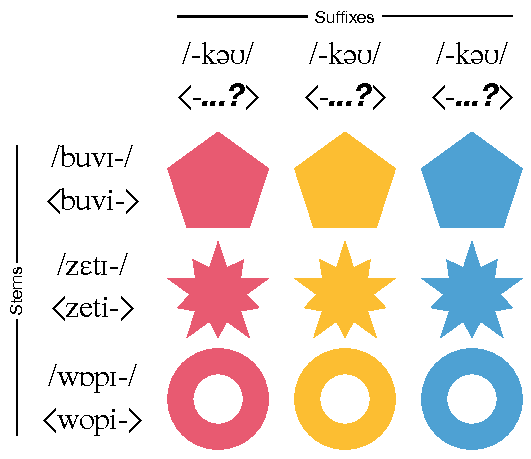
\includegraphics[scale=0.8]{figs/stimuli.pdf}}
	\vspace*{2pt}
	\caption{The nine object stimuli with their stems and suffixes. The spoken and written forms of the stems were fixed and unchanging throughout the experiment, as were the spoken forms of the suffixes, which were always homophonous; however, the written forms of the suffixes were free to evolve over time, potentially taking on differentiated forms to indicate color (e.g., <-co>, <-ko>, and <-qo> to represent pink, yellow, and blue).}
	\label{stimuli}
	\end{figure}

Participants were taught words for nine alien objects---three shapes (pentagon, star, torus) in three colors (pink, yellow, blue), as depicted in Fig.~\ref{stimuli}. The alien words had a spoken and written form composed of a stem and suffix. The stems, which always express the shape dimension, were /buvɪ/ <buvi> (the pentagon), /zɛtɪ/ <zeti> (the star), and /wɒpɪ/ <wopi> (the torus). These stems were fixed and unchanging throughout both experiments reported in this paper and were designed to be easy to learn by being graphically and phonetically iconic of the shapes they represent \newmaterial{(e.g., the round torus shape is represented by ``round'' sounds/letters)}. Throughout Experiment~1, the spoken form of the suffix was always pronounced /kəʊ/, but its spelling was free to change over time. Thus, the spoken form of the language consists of just three unique words---/buvɪkəʊ/, /zɛtɪkəʊ/, and /wɒpɪkəʊ/---that mark only a shape distinction; however, the spelling of the suffix could potentially take on different forms to mark color.

Each of the 10 transmission chains was seeded with a randomly-generated suffix spelling system, which was created by randomly mapping the following nine spellings onto the nine objects: <co>, <coe>, <coh>, <ko>, <koe>, <koh>, <qo>, <qoe>, <qoh>. In other words, the /k/ sound may be spelled <c>, <k>, or <q> and the /əʊ/ sound may be spelled <o>, <oe>, or <oh>, although the initial seed system contained no particular regularity. This procedure models an initial state of high spelling variation (every object has a unique suffix spelling), but these spellings may, over time, become transparent (the /k/ and/or /əʊ/ sounds take on consistent spellings) or expressive (spellings of /k/ and/or /əʊ/ become systematically associated with meaning). The spoken forms were synthesized using the Apple text-to-speech synthesizer (Tessa voice).

\subsubsection{Transmission procedure}

	\begin{figure}
	\makebox[\textwidth][c]{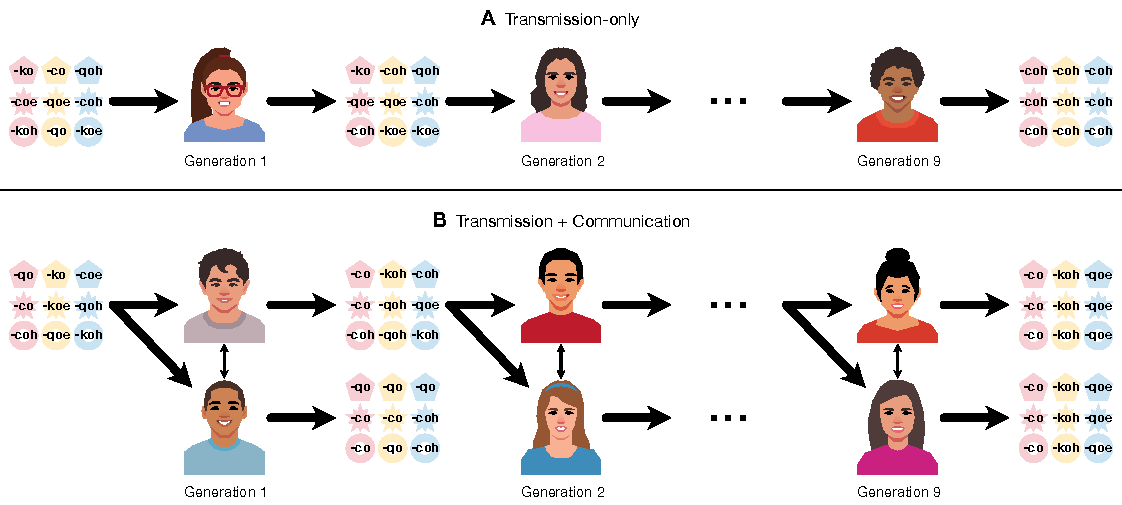
\includegraphics[scale=0.8]{figs/transmission.pdf}}
	\vspace*{2pt}
	\caption{\textbf{A} Transmission-only procedure. Each generation consists of a single participant, who first receives training on six of the nine suffixes and then produces suffixes for all nine items. These productions are then used as the training material for the next generation in the chain. The initial system of suffixes is randomly generated with high spelling variation; but by the ninth generation, the system is expected to become transparent. \textbf{B} Transmission~+ Communication procedure. Each generation now consists of two participants who engage in a communicative task. Both participants receive training on the same system from the previous generation. Under a communicative pressure, the suffix spellings are expected to become expressive of color, despite the spoken forms being homophonous.}
	\label{transmission}
	\end{figure}

Participants were arranged into transmission chains such that the spellings produced by one participant would subsequently be taught to the next participant in the chain (see Fig.~\ref{transmission}A). The first participant in a chain was taught the initial, randomly generated seed system, and this system was then free to evolve as it was transmitted to subsequent generations. Importantly, this process was subject to a bottleneck on transmission: Not all nine spellings were transmitted from one generation to the next; rather, the participant at generation $i$ would observe only six of the nine spellings produced at generation $i-1$ (at least one of each shape and at least one of each color).\footnote{\newmaterial{The 2/3 bottleneck parameter was chosen based on common practices in the field and some piloting. In general, increasing this parameter will lead to a slower evolutionary process, so the value was chosen to allow for sufficient change to occur within nine generations.}} Nevertheless, participants were asked to produce a spelling for all nine objects, meaning that generalization was required for three unseen items. Transmission continued for nine generations in each of ten independent chains. In the Transmission~+ Communication condition (see Fig.~\ref{transmission}B), each generation consisted of a pair of participants, but the productions of only one of the two (the primary participant; determined by whichever participant started the experiment first) were iterated to the next generation. The productions of the secondary participant were not iterated any further and were thus a cultural deadend; the role of the secondary participant was to act as a genuine communicative partner for the primary participant, inducing pressure for the language to become informative.

\subsubsection{Training procedure}

All participants were trained on the spoken and written forms through a combination of passive exposure trials and ``mini-test'' trials\newmaterial{, lasting around 8~min}. Participants were also told explicitly before starting the training session that the stems looked and sounded like the objects' shapes, allowing participants to focus on learning the suffixes during the training phase. In passive exposure trials, the alien objects were presented alongside the written and spoken forms in quick succession for 2~s each. In mini-test trials, which were interleaved among the passive exposure trials, the participant was asked to type the appropriate written form for an object and was given feedback on any errors (deleted characters shown in red strikethrough text and additions shown in bold green text). The participant received a 2p bonus for spelling the word correctly but had to submit their response within 20~s. Each of the six object--word pairs in the training set (i.e., the seen items that passed through the bottleneck on transmission) was passively exposed 18 times and mini-tested six times, resulting in a total of 108 passive exposure trials and 36 mini-test trials (the maximum bonus in training was therefore 72p). To check that participants were listening to the spoken forms, they were asked auditorily to click on the alien object at three random points during training; participants who did not follow this instruction were excluded. \newmaterial{The instructions provided to participants are provided in Appendix~A in the supplementary material.}

\subsubsection{Test procedure in Transmission-only}

After training, participants assigned to the Transmission-only condition completed a test phase, alternating between production and comprehension trials. In production trials, the participant was shown an object and heard its associated pronunciation. The participant's task was to type the appropriate spelling. The input box was limited to eight lowercase Latin characters, and participants had to spell the stem correctly to continue to the next trial. Since participants heard the word pronounced aloud, typing the stem correctly should have been trivial, but in cases where the stem was initially spelled incorrectly, a popup message explicitly reminded the participant of the correct spelling of the stem.\footnote{\newmaterial{Although artificial, these stem correction messages were rarely encountered. 81\% of participants never encountered this message (they always spelled the stem correctly), 14\% encountered it on one trial (out of nine), and 5\% encountered it on two or three trials.}} This restriction was imposed to prevent the stems from diverging from their spoken forms over time; however, no such restriction was imposed on the spelling of the suffix. Since the overall word length was restricted to eight characters and since all stems were four letters long, participants could use, at a minimum, a zero suffix and, at a maximum, a four-letter suffix. In comprehension trials, the participant was shown a word and had to click on the matching object from an array of all nine objects arranged in random order (in cases where multiple objects were described by the same wordform, any of the objects was a valid choice). In both types of test trial, the participant was awarded a bonus of 2p for each correct answer, but no explicit feedback was provided \newmaterial{on the correctness of the signal or object selection}. Each of the nine object--word pairs (i.e., including unseen items) was tested once in production and once in comprehension, resulting in 18 trials (the maximum bonus in test was therefore 36p).

\subsubsection{Test procedure in Transmission~+ Communication}

Participants assigned to the communicative condition completed a live, over-the-internet communication game with another participant. Both participants received training on the same orthographic system inherited from the previous generation.\footnote{\newmaterial{The seen items were selected independently for each participant. We felt this was more ecological than giving both participants identical input.}} The communication game, \newmaterial{which shares similarities with \textcite{Kirby:2015},} closely mirrored the overall structure of the test administered to participants in the non-communicative condition described above, with the production and comprehension trials becoming the two sides of a single communicative interaction. On a given trial, one participant (the director) would complete a production trial under the same input restrictions described above (i.e., produce a form for a target meaning), and the word they used was relayed to the other participant (the matcher), who would then complete a comprehension trial in response to that word (i.e., pick an object from the matcher array). The two participants then switched roles, resulting in the same overall trial structure as the Transmission-only condition (i.e., alternation between production and comprehension trials).

The framing and goal of the communication game was, however, quite different from the non-communicative test. In communication, the shared goal of the director and matcher is to have a successful communicative interaction, not necessarily to reproduce what they had learned in training. Both participants received the 2p bonus each time an interaction was successful; that is, the reward structure is not based on using the ``correct'' forms taught in training but based on accurately conveying meaning. The director is thus incentivized to produce a wordform that is unambiguous, and the matcher is incentivized to carefully interpret what the director has attempted to convey. The second important difference from the non-communicative test was that participants received rich feedback on the interaction: The director saw which object the matcher clicked on, and the matcher saw which object was the correct target. \newmaterial{As such, we view feedback as an intrinsic part of communicative interaction; thus, in the non-communicative test described above, no feedback was provided, as is the case in similar studies \parencite{Carr:2017, Motamedi:2019, Saldana:2019, Silvey:2019}.}

Overall, the communication game is identical to the non-communicative test in terms of the task to be performed (nine productions and nine comprehensions), but the goal is quite different. In the non-communicative test, the goal and reward structure are based on accurately reproducing the orthography learned during training, whereas in the communication game, the goal and reward structure are based on successfully communicating a target object.

\subsection{Results}

	\begin{figure}
	\makebox[\textwidth][c]{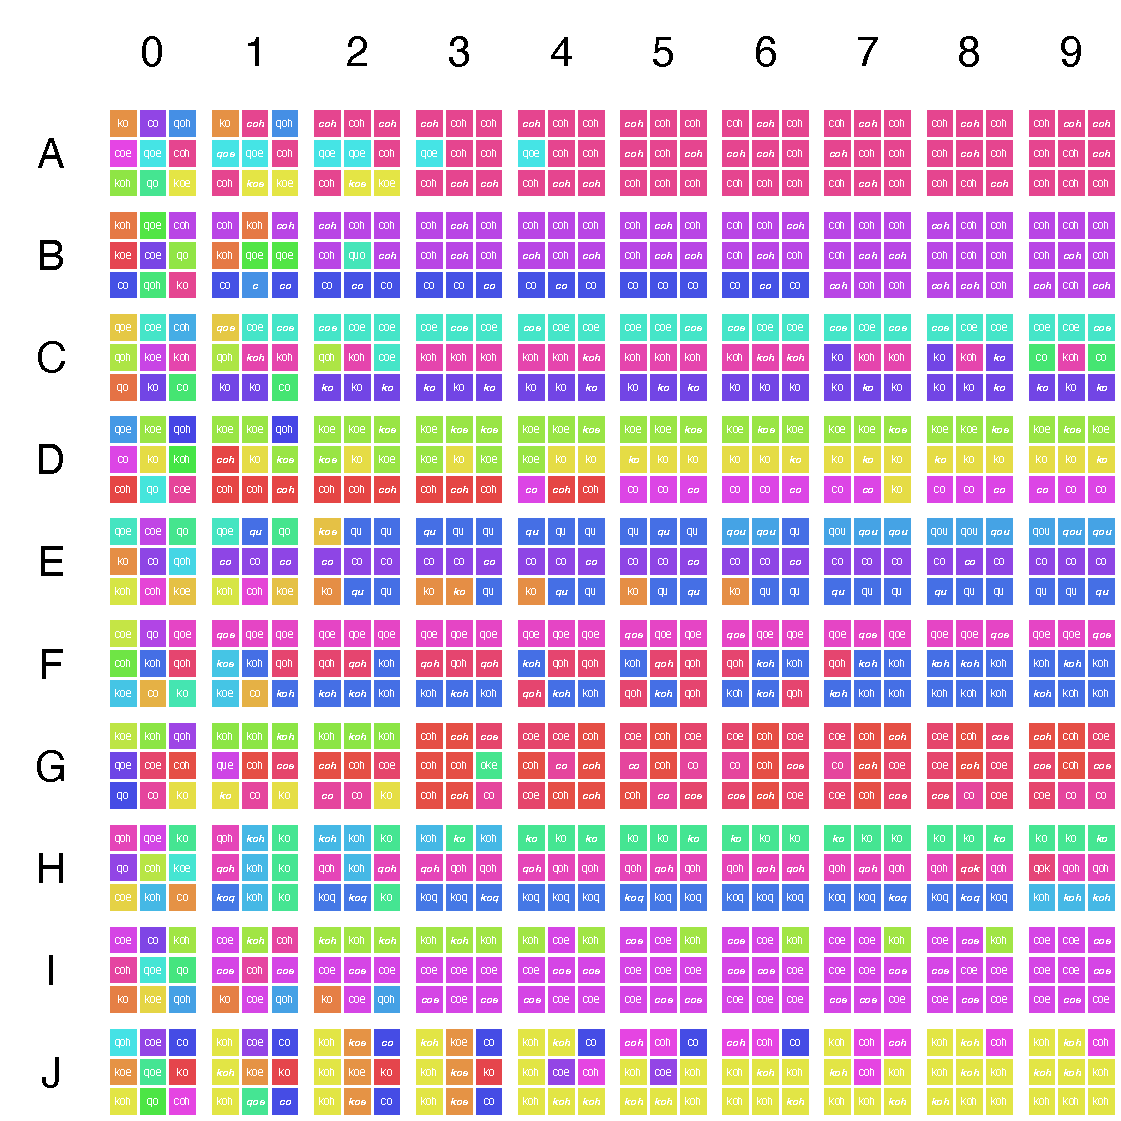
\includegraphics[scale=0.8]{figs/dif_lrn.pdf}}
	\vspace*{2pt}
	\caption{Results from the Transmission-only condition in Experiment~1 (differentiation). Each matrix shows the suffix spelling system in use at a particular generation (shape on the rows, color on the columns, as in Fig.~\ref{stimuli}). Chains are labeled A--J and generations are labeled 0–9 (0 is the randomly generated seed system). Each chain uses an independent color palette, with each color representing a particular suffix spelling; similar colors indicate similar spellings. Spellings in bold-italic are the generalizations on unseen items. By the ninth generation, most systems are degenerate (e.g., Chains~A, B, and~I), redundant (e.g., Chains~D, E, and~H), or a mixture of the two (e.g., Chain~F).}
	\label{dif_lrn}
	\end{figure}

The results from all ten chains (labeled A--J) in the Transmission-only condition are shown in Fig.~\ref{dif_lrn}. Each 3×3 matrix represents the suffix spelling system in use at a particular generation with shape represented along the rows and color represented along the columns, following the same 3×3 layout used in Fig.~\ref{stimuli}. The color-coding of these matrices indicates similarity in suffix form: Similar colors are used to represent similar suffixes, making it easier to see how the suffixes pattern with meaning.\footnote{The color-coding was generated independently for each chain by selecting $n$ evenly-spaced hues, where $n$ is the number of unique forms that emerged across the chain, and mapping these hues onto the suffixes in alphabetical order.} For example, the system at Generation~9 in Chain~D uses three spellings (<koe>, <ko>, and <co>) to express the shape dimension, yielding a horizontal stripes pattern in the matrix representation. We describe such a system as ``redundant'' because shape was consistently and reliably expressed by the stem, so the suffix spelling system that emerged in this case conveys no additional information---the suffix simply repeats whichever shape was marked by the stem. Redundant suffix systems are characteristic of the Transmission-only condition, with similar outcomes occurring in Chains~C, E, F, and~H. We also saw the emergence of fully transparent suffix spelling systems in Chains~A, B, I, and~J. Chain~I, for example, ultimately uses a single spelling, <coe>, to represent the /kəʊ/ sound; that is, the written suffix forms make no distinction between shapes or colors, just like the spoken language. Chain~G did not settle on a clear pattern, using <co>, <coe>, and <coh> somewhat interchangeably in the final generation, although there were some signs of a color-expressive system emerging in, for example, Generation~6, where yellow is consistently spelled <coh>, blue is consistently spelled <coe>, and pink uses both <co> and <coe>. The only other signs of color-expressive systems are H1, which was rapidly converted into a redundant system in subsequent generations, and J2, which ultimately degenerated toward transparency.

	\begin{figure}
	\makebox[\textwidth][c]{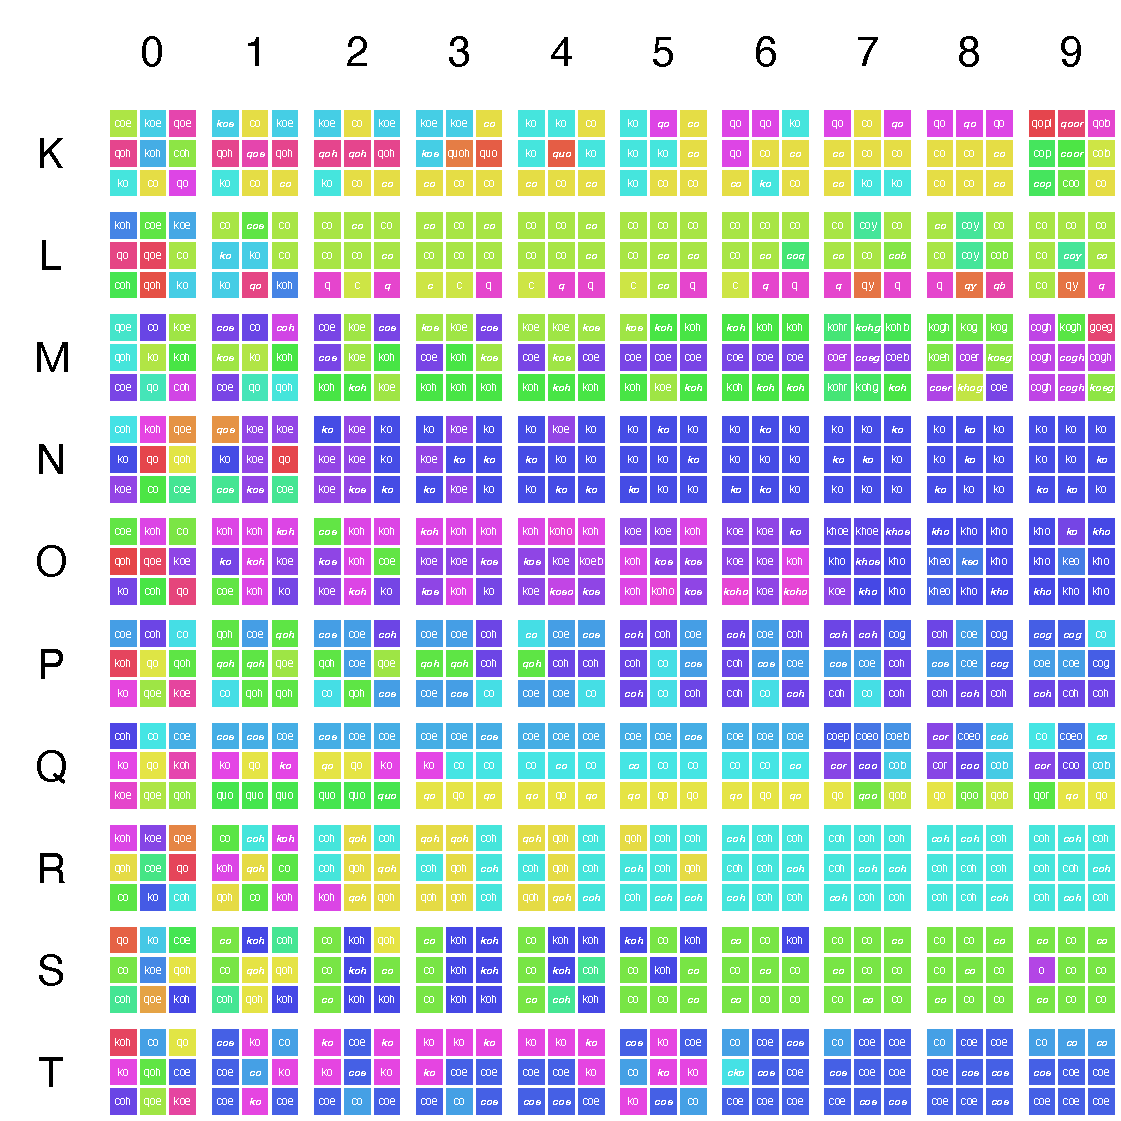
\includegraphics[scale=0.8]{figs/dif_com.pdf}}
	\vspace*{2pt}
	\caption{Results from the Transmission~+ Communication condition in Experiment~1 (differentiation). Each matrix shows the suffix spelling system in use at a particular generation (shape on the rows, color on the columns, as in Fig.~\ref{stimuli}). Chains are labeled K--T and generations are labeled 0–9 (0 is the randomly generated seed system). Each chain uses an independent color palette, with each color representing a particular suffix spelling; similar colors indicate similar spellings. Spellings in bold-italic are the generalizations on unseen items. There are some isolated examples of differentiation through implicit generalization (K5, M1, P5, S2) and explicit innovation (K9, L7, M7, O4, Q7).}
	\label{dif_com}
	\end{figure}

The results for the Transmission~+ Communication condition (Chains~K--T) are shown in Fig.~\ref{dif_com}. Like Transmission-only, degeneration to a single spelling by the ninth generation is a relatively common outcome (e.g., Chains~N, R, and~S and to a lesser extent Chains~L, M, and~O). In contrast, redundant, shape-expressive systems (as indicated by horizontal stripes) are relatively rare (e.g., K8, M6 and Q1--6). Instead, the presence of the communicative task appears to favor color-expressive systems, although these are far from common and often unstable. In particular, there are two main kinds of color-expressive system that emerge. The first are the generalization-based expressive systems: K5, M1, P5, and S2. In these cases, the participant tended to generalize their input in a way that is consistent with expressing color over shape. For example, in K5, pink was consistently spelled <ko> and blue was consistently spelled <co>. In the case of M1, color is expressed by the final vowel letters (<oe> for pink, <o> for yellow, and <oh> for blue) with the spelling of the /k/ sound conditioned on the stem (<buvic->, <zetik->, and <wopiq->). We note, however, that in all these cases the expressive system was not reciprocated by the participant's partner---resulting in low communicative accuracy---and not sustained or elaborated~on in subsequent generations.

The second type of color-expressive system is one that simply appropriates the expressive power of English to differentiate color: K9, M7, Q7, and to a lesser extent L7 and O4. In M7, for example, the participant added <r>, <g>, and <b> (presumably red, gold, blue) to the ends of the words, although the participant's partner only reciprocated the <g> spelling and seemingly failed to understand what was meant by <r> and <b>. In the case of Q7, the pair of participants added <r>, <o>, and <b> (presumably red, orange, blue) to communicate with high accuracy, but, although this system was retained into Generation~8, it started to disintegrate by Generation~9. Overall, in the five cases where English color letters were used, the systems did not really catch~on, perhaps because they retained spelling redundancy from the previous generation, resulting in unnecessarily complex suffix spellings that were too difficult to learn for subsequent generations. Q7, for example, uses <-coe->, <-co->, <-qo-> for shape plus <-r>, <-o>, <-b> for color. In addition to this handful of cases, there were a further four pairs of participants who used full English words as the suffix (typically <-pink> or <-red>, <-oran> or <-yell>, and <-blue>), but these pairs were excluded and replaced before iteration to the next generation.\footnote{In our preregistration, we stated that we would reject participants who used English color words. We allowed single letters because these were typically less transparent, especially in cases where the choice of letter (e.g., <g> or <r>) did not match how another person might have perceived the color (yellow vs.\@ gold vs.\@ orange or pink vs.\@ red). Indeed, as we see in the results, subsequent generations often did not pick~up~on the color letters (L9, M8, and Q9).} We mention these cases, however, because they are still examples of a conscious effort to differentiate---something that never happened in the Transmission-only condition.

	\begin{figure}
	\makebox[\textwidth][c]{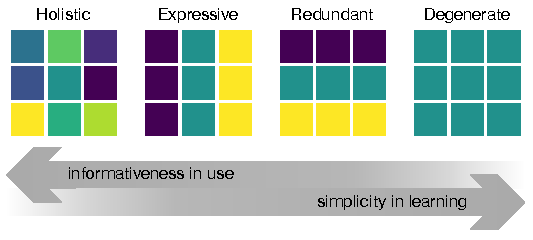
\includegraphics[scale=0.8]{figs/typology.pdf}}
	\vspace*{2pt}
	\caption{Four primary systems of interest (or typological categories) arranged along the cost/complexity continuum. A holistic system uses a unique suffix spelling for each shape--color combination. An expressive system only expresses color. A redundant system only expresses shape (which is already conveyed by the stem). A degenerate system expresses nothing.}
	\label{typology}
	\end{figure}

To analyze more formally what types of system tend to emerge under different conditions, we first designated four suffix systems that are of particular interest: holistic, expressive, redundant, and degenerate. These four typological categories may be positioned along the simplicity--informativeness continuum in terms of the number of suffix forms they make use of and how these forms are conditioned on meaning, as illustrated in Fig.~\ref{typology}. The holistic\footnote{Our use of the term \textit{holistic} is slightly unusual here, owing to the fact that we are focused on the suffix level and not the word level. By holistic, we only mean that each shape--color combination has a unique suffix form. We do not distinguish between truly holistic suffixes (nine unique suffixes with no structure in how they relate to each other) and compositional suffixes (nine unique suffixes that can be generated from compositional rules, as was the case in, for example, Q8).} system has nine unique forms each of which expresses a particular color--shape combination. This is complex to learn, but the suffix alone can pick out exactly one meaning. The expressive and redundant systems have three unique forms that express either color (expressive) or shape (redundant). These systems are easier to learn, but only the expressive system is fully informative (when acting in combination with the stem). The degenerate system uses just one suffix form. This makes it trivial to learn, but entirely uninformative. To classify a participant's output into one of these four typological categories, we computed which of the reference systems was most similar in terms of its information content. To do this, we formalized the systems as set partitions (i.e., a partitioning of the universe of meanings into disjoint subsets) with variation of information \parencite{Meila:2007} defined as the distance metric between any two such partitions.\footnote{Variation of information is a proper metric on set partitions, measuring the amount of information (in bits) that is lost and gained in the transformation of one partition into another. Under this metric, the holistic and degenerate systems are considered very dissimilar because they carry very different levels of information content. The expressive and redundant systems are also considered quite dissimilar because, although they carry the same amount of information, the information they carry is orthogonal (shape in the case of redundant, and color in the case of expressive).} A given participant's output system is then classified into one of the four typological categories based on whichever reference system is closest.

	\begin{figure}
	\makebox[\textwidth][c]{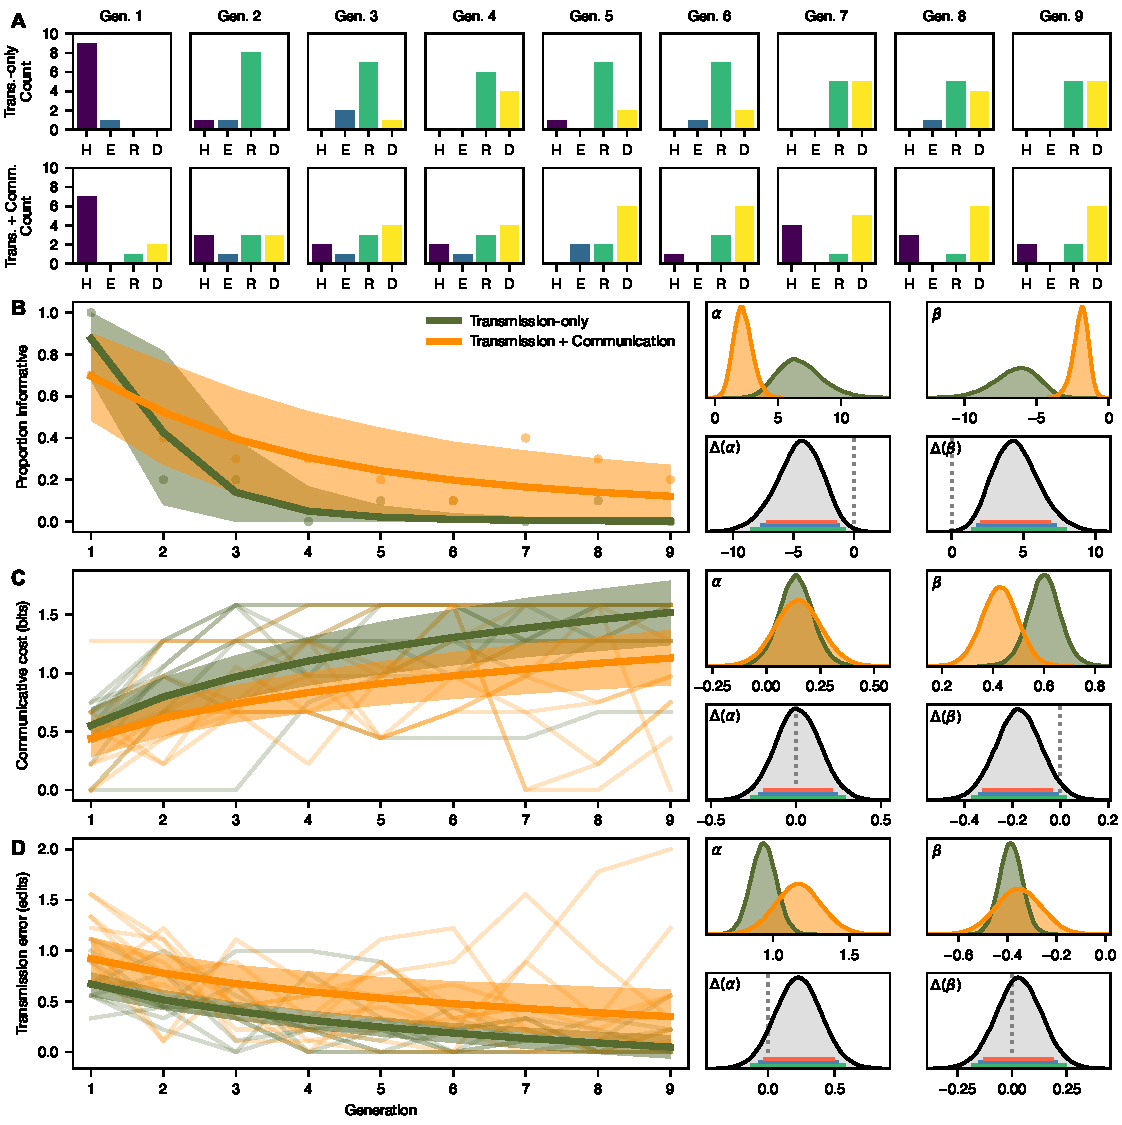
\includegraphics[scale=0.8]{figs/results_exp1.pdf}}
	\vspace*{2pt}
	\caption{Results of Experiment~1. \textbf{A} Typological distribution by generation and condition over the four typological categories: holistic (H; purple), expressive (E; blue), redundant (R, green), and degenerate (D; yellow). \textbf{B} Proportion of systems classified as informative (holistic or expressive) by generation. The dots show the observed proportions and the curves show logistic regression models fit to the data. \textbf{C} Communicative cost by generation along with regression models fit to the data. \textbf{D} Transmission error by generation along with regression models fit to the data. The panels on the right show the posterior estimates of the intercept ($\alpha$) and slope ($\beta$) parameters by condition as well as the posterior differences between conditions. The green, blue, and red bars indicate respectively the 95\%, 90\%, and 85\% HDIs (credible intervals).}
	\label{results_exp1}
	\end{figure}

The typological distributions are plotted in Fig.~\ref{results_exp1}A, revealing the proportion of the 10 chains that fall into each typological category at each generation. In Transmission-only, the holistic systems used to initialize the chains are rapidly replaced by redundant systems by Generation~2. The dominance of the redundant category is then gradually eroded as the chains transition to degeneracy. In Transmission~+ Communication, there is initially a fairly even mix of all four kinds of system, but by Generation~9, degenerate systems tend to be most common. There is also a notable increase in holistic systems emerging in later generations; these are the cases of compositional suffixes that arose through the addition of English color letters on top of redundant suffix spellings (i.e., K9, M1, M7, and Q7). Although there was not much evidence of expressive systems emerging in either condition, it is interesting to note that the communicative condition did seem to disfavor the inexpressive redundant systems.

\newmaterial{To analyze how informativeness changes over time and how this compares between the two conditions, we reduced the typological classifications into two broader categories: informative systems (i.e., holistic or expressive) and uninformative systems (i.e., redundant or degenerate). We then fit a Bayesian mixed-effects logistic regression model that predicts whether or not a system is informative as a function of generation with by-chain random slopes and intercepts,\footnote{Model: informative $\sim$ log(generation) + (1 + log(generation) | chain). Bernoulli likelihood with logit link function, weakly informative default priors, six chains of 12000 samples. All statistical models were fit using Bambi 0.13 \parencite{Capretto:2022}. Parameter estimates and diagnostics are provided in Appendix~B of the supplementary material.} which is the standard model structure used to analyze iterated learning experiments \parencite{Winter:2016}. Our Bayesian approach produces posterior estimates of two key parameters: $\alpha$, representing the intercept of the regression model, and $\beta$ representing its slope. To determine if there is a statistical difference between conditions, we compute the difference in slopes, $\Delta(\beta) = \beta_\mathrm{comm} - \beta_\mathrm{trans}$, and check if this posterior difference satisfactorily rejects zero. Here we follow the convention that the 95\% highest density interval (HDI; the narrowest interval that contains 95\% of the posterior probability mass) should not include zero. We emphasize, however, that the posterior is a complete description of the evidence (given the data and model assumptions) and does not strictly need to be reduced to a binary yes/no decision. The results are shown in Fig.~\ref{results_exp1}B. In both conditions, there is a decrease in informativeness over time (the slopes are negative), but in the Transmission + Communication condition, the slope is shallower, suggesting that informativeness decreases more slowly in the presence of communicative pressure. The difference in slopes, $\Delta(\beta) = 4.53$ (95\%~HDI: 1.48, 7.88), clearly rejects zero, pointing to a meaningful difference between conditions.}

\newmaterial{One issue with the above approach is that collapsing the systems into binary categories (informative vs.\@ uninformative) results in a loss of information about \textit{how informative} the systems are. In addition, there was evidence to suggest that the model was a suboptimal description of the data, since there was also a difference in the $\alpha$ estimates (the intercepts), which should theoretically be the same (i.e., there should be no difference between conditions at Generation~0). We address these limitations with a second measure of informativeness, communicative cost \parencite{KempRegier:2012, Kemp:2018, Regier:2015}, which has previously been used in similar experimental studies \parencite{Carr:2020, Carstensen:2015, Smith:2020} and was proposed in our preregistration as the primary measure of informativeness.} Communicative cost is an information-theoretic measure that expresses how much information will be lost, on average, when a speaker/writer attempts to convey a meaning to a listener/reader using some shared signaling system. If the system contains no ambiguities (all meanings are expressed by unique signals), communicative cost will be zero~bits---that is, zero information will be lost during each attempt to communicate using that system. Communicative cost will take some larger value if the system contains ambiguity. It is given by $\sum_{m \in U} \mathrm{Pr}(m) ( -\log \mathrm{Pr}(m|s_m) )$, where $U$ is the universe of meanings that may be expressed, $\mathrm{Pr}(m)$ is the probability that a particular meaning would need to be expressed, and $\mathrm{Pr}(m|s_m)$ is the probability that a reader would infer meaning $m$ given that a writer produced signal $s$ for meaning $m$. In our case, $U$ is the set of nine alien objects, $\mathrm{Pr}(m)$ is set to $1/|U|$ (all objects need to be talked about with equal probability), and $\mathrm{Pr}(m|s_m)$ is given by $1/|M_s|$, where $M_s$ is the set of meanings labeled $s$ according to the system. \newmaterial{The results are shown in Fig.~\ref{results_exp1}C. We used the same mixed-effects linear regression model described above (except that the likelihood is now Gaussian). In line with the previous analysis, cost increases with generation in both conditions but increases more slowly under communicative pressure. However, the support for a difference between conditions was weaker under this more nuanced measure, $\Delta(\beta) = -0.17$ (95\%~HDI: $-0.36$, $0.02$); although we were not able to reject zero at the 95\% level, we were able to reject it at the 92\% level (92\%~HDI: $-0.35$, $-0.01$).}

\newmaterial{Aside from the informativeness of the orthographic systems, we also predicted in our preregistration that the systems would become easier to learn over time in both conditions, albeit for slightly different reasons. In Transmission-only, the orthographic system is expected to become increasingly learnable as it degenerates into a single, transparent suffix form. In Transmission~+ Communication, the system is expected to become more learnable as the unsystematic, holistic systems transform into other easier to learn systems (notably expressive systems, although---as noted already---expressive systems rarely emerged). Following prior work, we operationalized learnability as transmission error---the amount of error that the participant at Generation~$i$ made in reproducing the orthographic system that existed at Generation~$i-1$; transmission error is defined as the mean Levenshtein edit distance between the corresponding orthographic forms in consecutive generations \parencite[see e.g.,][]{Kirby:2008}. These results are plotted in Fig.~\ref{results_exp1}D. In both conditions, the estimates of the $\beta$ parameters are negative and clearly reject zero, suggesting that the systems do indeed become increasingly learnable over time. There was some weak evidence for a difference in the intercepts, with transmission error remaining higher in the communicative condition. This is to be expected because the goal in the Transmission-only condition is to reproduce the forms taught in training, whereas the goal in the communicative condition is to devise a system that permits accurate communication, which necessitates more change to the system that was learned.}

\subsection{Summary}

Our first experiment tested whether informative, heterographic orthography could emerge through spelling differentiation and whether it would emerge preferentially under communicative pressure. Although there was evidence to suggest that the orthographic systems remain informative for longer under communicative pressure, both conditions ultimately converged on degenerate, uninformative systems and there was little evidence of systematic differentiation in spelling. Other than resorting to English, such differentiation could have been achieved in a number of ways, most obviously through the conditioning of spelling variation on meaning (e.g., <ko> for pink, <co> for yellow, and <qo> for blue), but also through less obvious strategies such as the use of length (e.g., <ko> for pink, <kko> for yellow, and <kkko> for blue) or the use of arbitrary silent letters (e.g., <kox> for pink, <kof> for yellow, and <kom> for blue). Such differentiation was not forthcoming, however, even under communicative pressure. Instead, if spelling variation was conditioned on anything, it was conditioned on shape, resulting in redundant suffix spellings. This result is in stark contrast to most prior experimental iterated learning studies, in which informative, compositional systems do typically emerge, especially under communicative pressure \parencite[e.g.,][]{Kirby:2015}.

So, what was different about the present experiment compared to the large body of prior experimental iterated learning studies? The primary difference was the presence of a spoken language that is decidedly \textit{not} informative about one of the dimensions. Indeed, the point of our experiment is to see whether orthography can resist phonology under sufficient pressure for informativeness. The presence of homophonous suffix forms acts as a cue to participants that the language itself does not mark color and that, therefore, the orthography should also not mark color. \newmaterial{In support of this explanation, we conducted an additional experiment during review, which showed that when homophony is removed, the systems tend to resist degeneration in line with prior work. We discuss this experiment in more detail in the Discussion section and in Appendix~C of the supplementary material.}

Faced with orthographic variation that could be conditioned on either dimension, learners appear to rule out the possibility that it might be conditioned on color, since such a hypothesis would be in conflict with the spoken language. As a result, any variation in spelling comes to be associated with particular stems, resulting in the emergence of redundant suffix spellings that serve no real purpose. \newmaterial{Similar outcomes have been noted before in the context of artificial language learning experiments \parencite{Smith:2010},} and a rough analog can be found in English in the spelling of /-ʃən/ (<cian>, <cion>, <sion>, <ssion>, or <tion>), which is conditioned on the stem (e.g., \textit{magician} \textit{suspicion}, \textit{expulsion}, \textit{transmission}, and \textit{station}) following a complex set of rules \parencite[pp.~420--421]{Carney:1994}. \newmaterial{Interestingly, however, these redundant systems were relatively uncommon under communicative pressure, suggesting that communicating participants recognized the futility of using the suffix to mark shape.}

Overall, although the orthographic systems tended to remain slightly more informative under communicative pressure, the emergent orthographies ultimately preferred to transparently encode sound rather than meaning. This finding seems to align with our general experience of the world: If someone decided to start using the spelling <banque> to differentiate the financial institution from river banks, would anyone take that spelling seriously or even understand the intention? Without top-down diktat, it is hard to get spelling differentiation off~the~ground in the written modality.

%~%~%~%~%~%~%~%~%~%~%~%~%~%~%~%~%~%~%~%~%~%~%~%~%~%~%~%~%~%~%~%~%~%~%~%~%~%~%~%~%~%~%~%~%~%~%~%~%~%~%~%

\section{Experiment 2}

We now turn our attention to the conservation model of heterographic homophones: Given that an informative system already exists (both in speech and in writing), does that informative system persist in writing even after the spoken language has degenerated into homophony? And, importantly, does this happen preferentially in the presence of communicative pressure? Our hypotheses were as follows:
\begin{enumerate}
	\item Under pressure from learning alone, we expect to find that orthography will track the spoken form of the language, becoming increasingly degenerate as homophony increases.
	\item Under additional pressure for disambiguation, we expect the orthography to conserve archaic (but informative) spelling distinctions even after these distinctions cease to exist in the spoken form of the language.
\end{enumerate}

\subsection{Methods}

The methods were identical to Experiment~1 with two exceptions: The artificial language used to seed each chain started out fully compositional (in both its spoken and written forms), and two sound mergers were artificially induced during cultural transmission, resulting in the spoken forms of the suffixes becoming increasingly homophonous and uninformative over time. This was designed to model the historical processes of sound change and conservation described in the Introduction.

\subsubsection{Participants}

The experiment was completed by 297 native-English participants recruited through Prolific. The payment and bonusing scheme was identical to Experiment~1 (median bonus: £0.78). The median completion time was 15~m with a median hourly rate of £7.99 (£10.68 including bonus). 17 participants were excluded because they (or their partners) failed the auditory attention checks (15) or used English color words (2). A further 10 participants were lost to communication-game pairing failures. Like Experiment~1, the final dataset comprises 270 participants: 90 in the Transmission-only condition (10 chains of 9 participants) and 180 in the Transmission~+ Communication condition (10 chains of 9 pairs of participants).

\subsubsection{Stimuli}

The alien objects and word stems were identical to Experiment~1. Unlike Experiment~1, however, the transmission chains were seeded with a fully compositional language that used three distinct suffixes to systematically express each of the colors. A separate set of suffixes was created for each chain by concatenating a randomly drawn consonant from \{/f/, /s/, /ʃ/\} and a randomly drawn vowel from \{/ə/, /ɛɪ/, /əʊ/\}, both without replacement. For example, one chain might use the suffixes /fəʊ/, /ʃə/, /sɛɪ/ to represent the colors pink, yellow, and blue, while another chain might use /sə/, /fɛɪ/, /ʃəʊ/ for those colors. The initial orthographic system was transparent and based on the following phoneme–grapheme mapping: \{/f/→<f>, /s/→<s>, /ʃ/→<x>, /ə/→<a>, /ɛɪ/→<ei>, /əʊ/→<oe>\}. The suffixes were designed to be distinctive (and therefore easy to memorize and associate with colors), but also similar enough to (mostly) allow for somewhat plausible sound mergers and result in somewhat plausible spellings following sound merger (e.g., it is plausible that /f/ might supplant /s/ or /ʃ/ in speech or that /ʃ/ might be spelled <s> or <x> in writing). We attempted to achieve this balance by combining consonants that are very similar with vowels that are very dissimilar, while also avoiding reuse of any sounds present in the stems. The spoken forms were synthesized using the Apple text-to-speech synthesizer (Moira voice).

\subsubsection{Sound change}

	\begin{figure}
	\makebox[\textwidth][c]{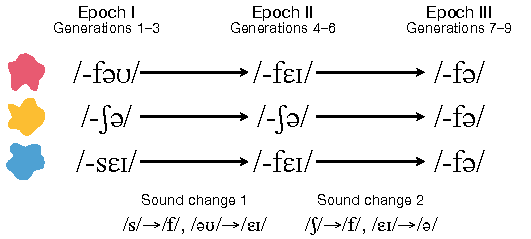
\includegraphics[scale=0.8]{figs/sound_change.pdf}}
	\vspace*{2pt}
	\caption{Examples of the spoken suffixes in Experiment~2. During Epoch~I, color is represented by three distinct spoken suffixes. During Epoch~II, two of the suffixes are homophonous, reducing the informativeness of the spoken language. During Epoch~III, the spoken form of the language makes no color distinction.}
	\label{sound_change}
	\end{figure}

Each transmission chain was run for nine generations, which were divided into three epochs. During Epoch~I (Generations~1 to~3), the three spoken suffixes were distinct (as described above), allowing the spoken language to express all three colors without ambiguity. During Epoch~II (Generations~4 to~6), the spoken language had two distinct suffix forms, reducing its informativeness. During Epoch~III (Generations~7 to~9), all three spoken suffixes were homophonous, just as in Experiment~1, making the spoken language entirely uninformative about color. This was achieved through two sets of sound changes, the first occurring in the transition from Epoch~I to~II and the second occurring in the transition from Epoch~II to~III. An example is illustrated in Fig.~\ref{sound_change}. In the first sound change, two of the spoken suffix forms were chosen at random and the consonant from one (chosen at random) was paired with the vowel from the other, resulting in a new suffix form that replaced the original two. In the second sound change, the remaining two suffix forms were merged in the same way, resulting in full homophony. Crucially, the spellings did not automatically change following a sound change event; rather, the orthographic system was free to adapt (or not) in response to the sound changes. Note also that individual participants did not directly experience the sound changes; a Generation~4 participant, for example, would always hear Epoch~II sounds, while observing spellings produced by a Generation~3 participant (presumably representing the Epoch~I sounds). In reality, of course, sound change is more gradual, with individual speakers experiencing both outgoing and incoming spoken forms within their lifetimes.

\subsection{Results}

	\begin{figure}
	\makebox[\textwidth][c]{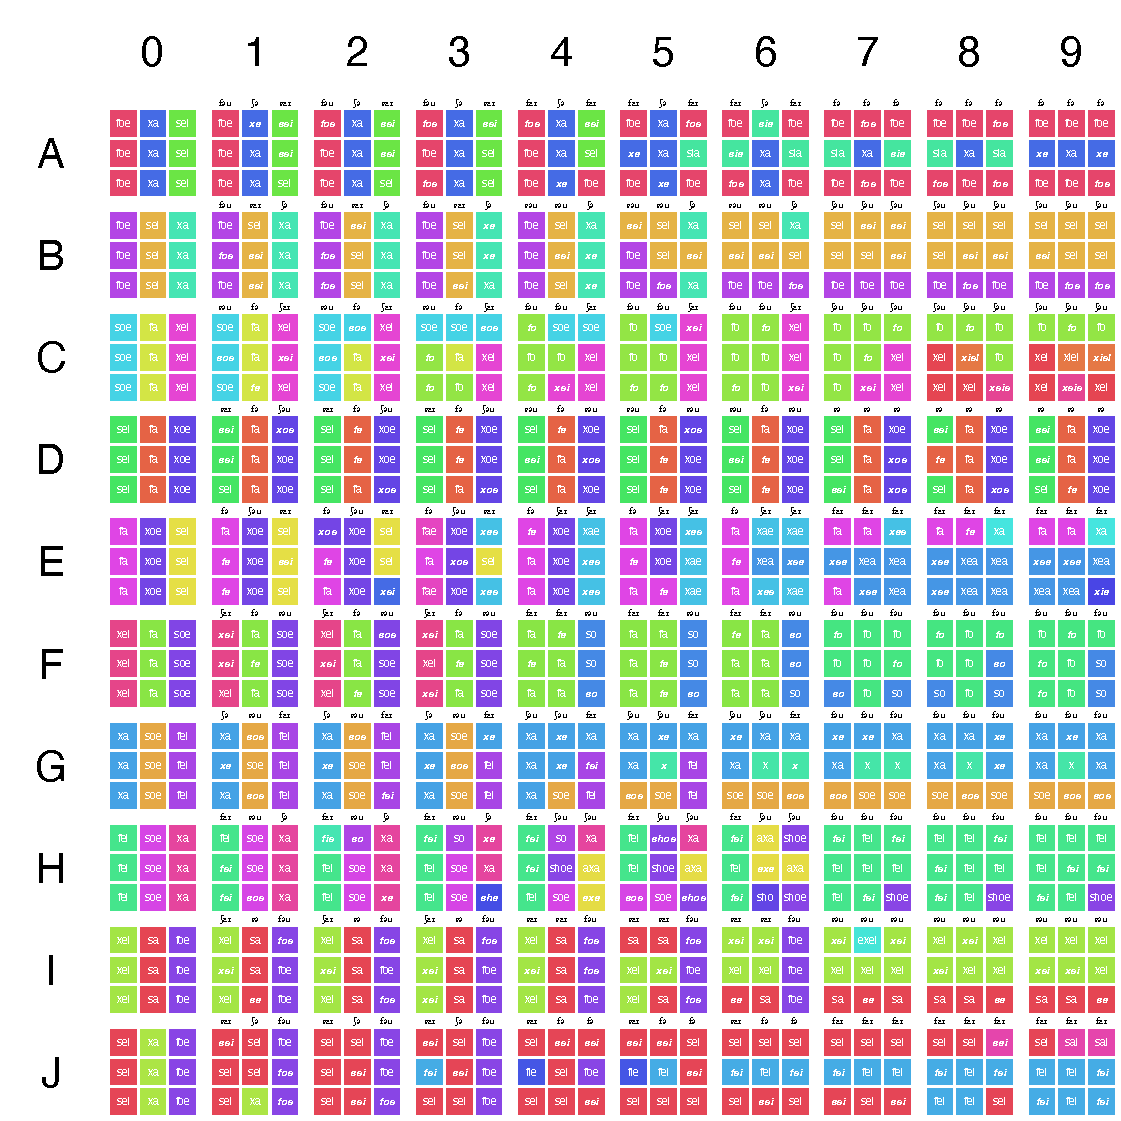
\includegraphics[scale=0.8]{figs/con_lrn.pdf}}
	\vspace*{2pt}
	\caption{Results from the Transmission-only condition in Experiment~2 (conservation). Each matrix shows the suffix spelling system in use at a particular generation (shape on the rows, color on the columns, as in Fig.~\ref{stimuli}). Chains are labeled A--J and generations are labeled 0–9 (0 is the randomly generated seed system). Each chain uses an independent color palette, with each color representing a particular suffix spelling; similar colors indicate similar spellings. Spellings in bold-italic are the generalizations on unseen items. The final systems are characterized by the conservation of form without the conservation of expressivity.}
	\label{con_lrn}
	\end{figure}

The results for all ten chains (labeled A--J) in the Transmission-only condition are shown in Fig.~\ref{con_lrn}. It is immediately clear that color-expressive suffixes (as indicated by vertical stripes) are maintained fairly reliably through the first epoch; perfectly in the case of Chains~A, B, D, F, and~I, and with some errors in the other five chains. Some of these errors are very minor, such as the use of <sha> instead of <xa> for one item in H3, while others are more catastrophic, such as the early loss of the <sei>/<xa> distinction in Chain~J. Generation~4 represents the first real test of the orthographic systems in the face of sound change, and, in most cases, the Generation~3 systems are preserved quite faithfully (Chains~A, B, D, E, H, and~I), but by the end of the epoch (Generation~6), many have degenerated into redundant systems that encode shape (Chains~B, G, and~J) or transparent systems that mirror the Epoch~II pattern of homophony (Chains~C, E, F, and~I). These processes continue into Epoch~III and by the ninth generation, all systems have become degenerate, redundant, or some mixture of the two. The one exception is Chain~D, whose original spellings were conserved perfectly through to the final generation with only one generalization error in Generation~8, which was quickly reverted in Generation~9.

Like Experiment~1, redundant systems are characteristic of the Transmission-only condition, especially in Epoch~III. As the spoken suffixes become more homophonous, the variant spellings are increasingly conditioned on shape rather than color, perhaps because the spoken language signals to learners that the language does not mark color, so they rationalize the system as three words with idiosyncratic spellings. Interestingly, however, all chains exhibited conservation of spelling \textit{form}, even if the way in which spelling was conditioned on meaning was lost. For example, Chain~A ultimately represents the sound /fə/ with the spellings <foe> and <xa>, spellings that are internally inconsistent and contrary to standard uses of the Roman alphabet, but which trace their origins back to the original seed orthography. Overall, then, the Transmission-only condition in Experiment~2 is characterized by the conservation of spelling \textit{form} without conserving how form patterns with meaning.

	\begin{figure}
	\makebox[\textwidth][c]{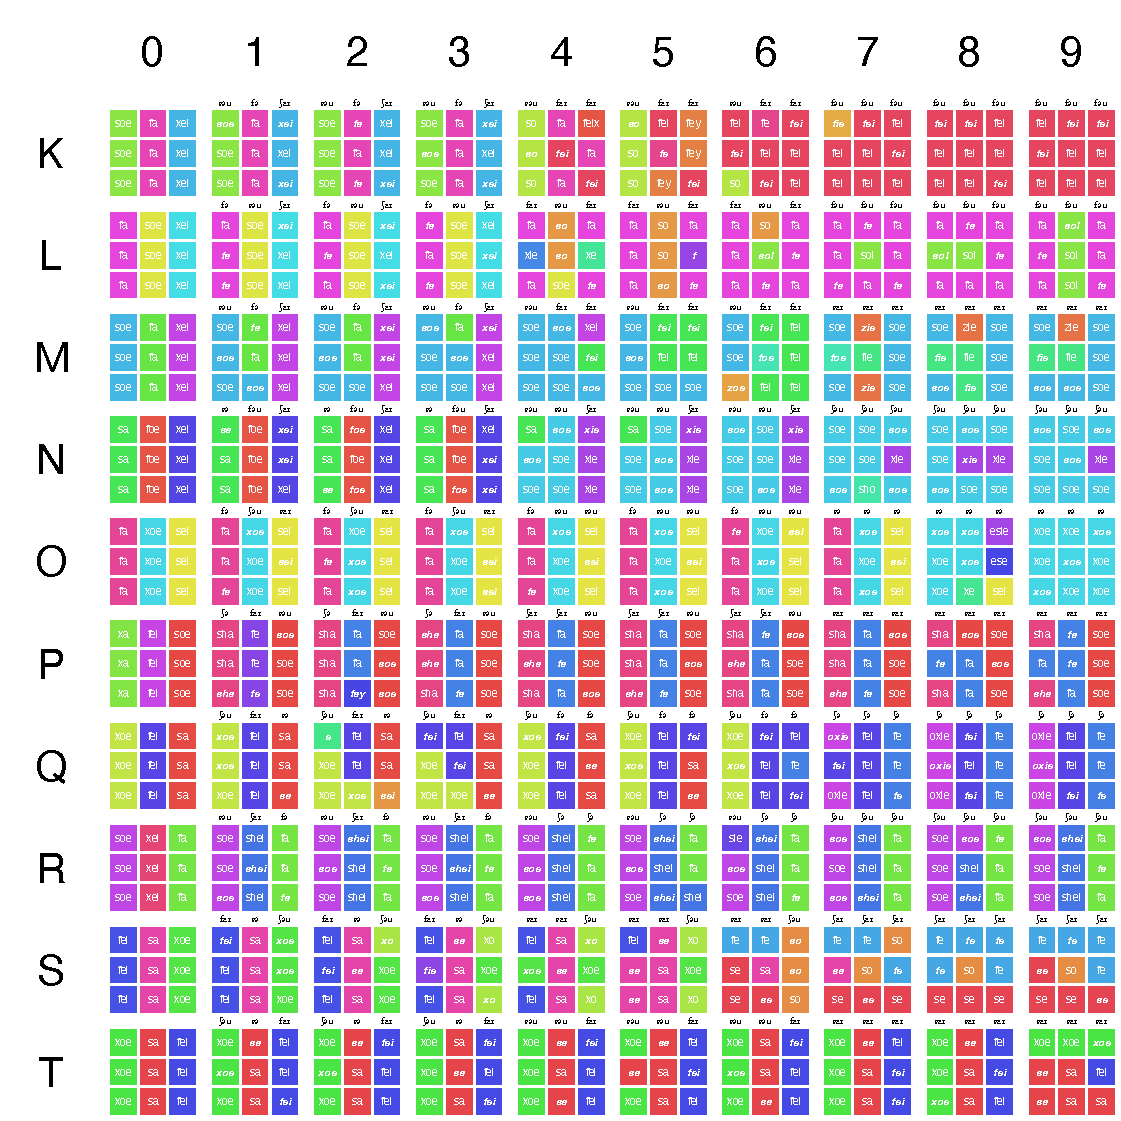
\includegraphics[scale=0.8]{figs/con_com.pdf}}
	\vspace*{2pt}
	\caption{Results from the Transmission~+ Communication condition in Experiment~2 (conservation). Each matrix shows the suffix spelling system in use at a particular generation (shape on the rows, color on the columns, as in Fig.~\ref{stimuli}). Chains are labeled K--T and generations are labeled 0–9 (0 is the randomly generated seed system). Each chain uses an independent color palette, with each color representing a particular suffix spelling; similar colors indicate similar spellings. Spellings in bold-italic are the generalizations on unseen items. Five chains (O, P, Q, R, T) remain fully expressive into the final epoch, in most cases conserving the original forms.}
	\label{con_com}
	\end{figure}

The results for the Transmission~+ Communication condition (Chains~K--T) are shown in Fig.~\ref{con_com}. Like Transmission-only, the seed systems are mostly maintained faithfully through Epoch~I; perfectly in the case of Chains~K, L, N, O, and~T, and with some errors in the other five chains, although some of these errors are non-destructive changes, such as <x> being replaced with <sh> in R1. Several systems were then maintained through Epoch~II, notably Chains~O, P, R, and~T, and, in one case, through to the end of Epoch~III (Chain~R, albeit with the original <xei> spelling replaced with <shei>). The Chain~O system was preserved up to Generation~7, Chain~P was maintained up to Generation~7 and almost to Generation~9 with two modifications (<sha> instead of <xa> and <fa> instead of <fei>), and Chain~T was conserved faithfully up to Generation~8. The final form of Chain~Q was also fully expressive, albeit through a combination of both conservation and differentiation: The <fei> form was conserved from the seed orthography, the <oxie> spelling appears to derive from a misremembering of <xoe> (partial conservation), and the <fe> spelling, which began as a typo introduced in Q6, seems to have been generalized across the blue items in Q7, perhaps to differentiate them from the yellow items (indeed, the participant's partner made the same generalization). A similar case of differentiation might also have occurred in L9, where the <sol> spelling (originally a typo on <so>) was generalized across the yellow items, resulting in a semi-expressive system (although the participant's partner generalized the <sol> spelling across shape).

Unlike Experiment~1, no participant pairs attempted to use English color letters and there was only one case of a pair using English color words (Generation~9 of Chain~K), although this pair was excluded and replaced (this generation was the only case in which the training input was fully degenerate, which would have resulted in a strong pressure to find a communicative solution in the form of English). Presumably, the general conservation of expressive spelling in Experiment~2 negated the need to innovate novel systems.

	\begin{figure}
	\makebox[\textwidth][c]{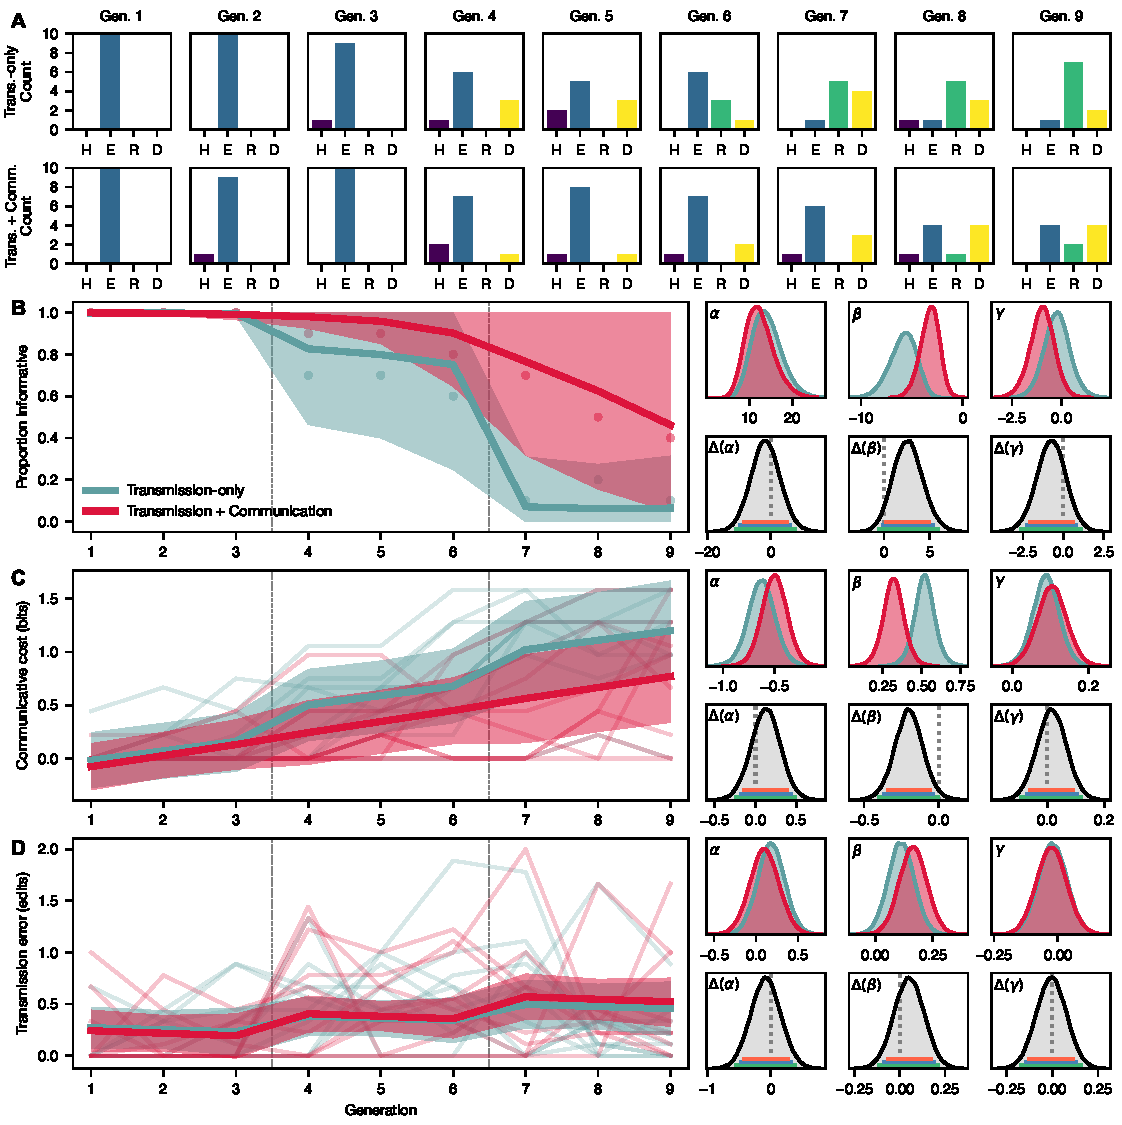
\includegraphics[scale=0.8]{figs/results_exp2.pdf}}
	\vspace*{2pt}
	\caption{Results of Experiment~2. \textbf{A} Typological distribution by generation and condition over the four typological categories: holistic (H; purple), expressive (E; blue), redundant (R, green), and degenerate (D; yellow). \textbf{B} Proportion of systems classified as informative (holistic or expressive) by generation. The dots show the observed proportions and the curves show logistic regression models fit to the data. \textbf{C} Communicative cost by generation along with regression models fit to the data. \textbf{D} Transmission error by generation along with regression models fit to the data. The panels on the right show the posterior estimates of the intercept ($\alpha$) and slope ($\beta$ and $\gamma$) parameters by condition as well as the posterior differences between conditions. $\beta$ represents the effect of epoch and $\gamma$ represents the effect of generation number within epoch. The green, blue, and red bars indicate respectively the 95\%, 90\%, and 85\% HDIs (credible intervals).}
	\label{results_exp2}
	\end{figure}

\newmaterial{Our quantitative analysis of Experiment~2 is identical to that of Experiment~1 with a slight change to the statistical model. Rather than predict the outcome variables as a function of generation, we now predict the outcome variables as a function of the epoch number (1, 2, or 3) and the generation number within the epoch (1, 2, or 3).\footnote{Model: dependent $\sim$ epoch + (1 + epoch | chain) + generation\_in\_epoch + (1 + generation\_in\_epoch | chain).} This yields two slope parameters: $\beta$, which represents the effect of epoch, and $\gamma$, which represents the additional effect of generational turnover. This model is more appropriate to the Experiment~2 setup, where the experimentally induced homophony results in discontinuities from one epoch to the next, and it allows us to separate out the effect of the homophony pressure from the more general effect of generational turnover.}

Fig.~\ref{results_exp2}A plots the typological distributions by generation and condition. Initially, all systems are expressive, but the dominance of this category is gradually eroded over time, particularly during the second and third epochs once the spoken forms had become homophonous. Notably, however, the loss of expressive systems appears to be slower in Transmission~+ Communication, and redundant systems were also less popular under communicative pressure. \newmaterial{As in Experiment~1, we further collapsed the typological categories into two broader categories (informative vs.\@ uninformative) to analyze the trends over time. The results, shown in Fig.~\ref{results_exp2}B, show that the probability of a system being informative drops over time in both conditions (primarily as a function of epoch), but does so more slowly in the communicative condition. Although there was some weak evidence of a difference in epoch slopes ($\Delta(\beta) = 2.65$; 95\%~HDI: $-0.58$, $5.95$), we could not conclusively reject zero under this measure.}

\newmaterial{The results in terms of the preregistered measure of informativeness, communicative cost, are presented in Fig.~\ref{results_exp2}C. Here we find a nonzero effect of both epoch and generation on cost, as well as a difference between conditions in terms of epoch: $\Delta(\beta) = -0.2$ (95\%~HDI: $-0.4$, $-0.003$). Like the previous analysis, the $\gamma$ slopes were in close alignment. This suggests that the effect of generational turnover is very similar between conditions and that the difference between conditions is mostly driven by the increases in homophony induced in each epoch. The overall result is that, in Transmission~+ Communication, the increase in cost is linear across the nine generations, whereas in the Transmission-only condition, the increase in cost follows something more akin to a step function, with sudden increases in cost in response to each additional bout of homophony. In other words, in the Transmission-only condition, the orthographic systems respond rapidly to the changing spoken forms, while in the Transmission~+ Communication condition, the orthographic systems are more resistant to the homophony.}

\newmaterial{For completeness, Fig.~\ref{results_exp2}D also plots transmission error; however, we did not hypothesize any particular differences in learnability in Experiment~2, either over time or by condition. The expressive orthographic systems used to initialize the chains start out very easy to learn, and learnability remains fairly consistent throughout the experiment in both conditions, albeit with some constant level of change over time as the systems gradually come into alignment with the spoken forms.}

\subsection{Summary}

Experiment~1 asked whether an informative, heterographic orthography may be \textit{created} de~novo under pressure from homophony. Experiment~2, by contrast, asked whether an informative, heterographic orthography can simply be \textit{maintained}, even under the same levels of homophony encountered in Experiment~1. In the Transmission-only condition, only one chain (Chain~D) remained expressive into the fully homophonous Epoch~III, while in Transmission~+ Communication, five chains (O,~P, Q, R, and~T) remained expressive, albeit not necessarily all the way to Generation~9. The fact that expressive spellings persisted longer and across more chains under communicative pressure suggests that an informative orthography---despite running contrary to the spoken language---may be maintained when it serves a useful purpose. That being said, the fact that informativeness could, in~principle, be maintained without communicative pressure (most notably in Chain~D) suggests that a strong communicative pressure is not a strictly necessary condition for conservation: Learning alone can, to a limited extent, maintain informative heterography.

Many of the chains did, however, eschew informativeness entirely in favor of greater transparency, and the inevitable long-term consequence for all chains appears to be degeneracy. This is to be expected under Transmission-only, where the systems are adapting under learnability pressure, but is somewhat surprising in Transmission~+ Communication. Our findings ultimately suggest that, in the long term, alphabetic orthographic systems might favor the faithful encoding of speech over the useful encoding of meaning, although there may exist brief windows of time during which informative heterography can resist the spoken language. Interestingly, although participants were resistant to encoding into writing something that is not encoded in speech, they were---at the same time---content to conserve spelling forms that were internally inconsistent and unusual. Tradition has a powerful hold over writing systems.

%~%~%~%~%~%~%~%~%~%~%~%~%~%~%~%~%~%~%~%~%~%~%~%~%~%~%~%~%~%~%~%~%~%~%~%~%~%~%~%~%~%~%~%~%~%~%~%~%~%~%~%

\section{Discussion}

The written and spoken forms of a language are never perfectly identical; they diverge in many ways as a result of the differing constraints relevant to each. Spacing between words for example does not exist in speech but constitutes a useful innovation in writing that permits rapid reading \parencite{RaynerFischer:1998, Sainio:2007, Zang:2013}. Similarly, the consistent spelling of affixes, such as the English past-tense marker <-ed>, which diverges from its spoken realization (/-d/, /-t/, or /-ɪd/ depending on the preceding sound), permits faster access to meaning \parencite{Ulicheva:2020}. Might it be the case that---left to evolve freely---the written form of a language will become better adapted to the needs of writers and readers to the detriment of its alignment with the spoken form of the language? Do writing systems adapt to the affordances and constraints of the written modality \parencite{Rastle:2019}?

We addressed these questions by focusing on the particular case of heterographic homophones---morphemes that sound the same but that are spelled differently. Heterographic homophones permit the written language to be more informative than the spoken language; the spellings <knight> and <night>, for example, convey a distinction in meaning that cannot be conveyed in speech without supplying additional information. We investigate whether heterography might arise for functional reasons by experimentally simulating the cultural evolution of orthography under two distinct mechanisms, differentiation and conservation, as described by \textcite{Berg:2021}.

\subsection{Experiment 1: Differentiation}

In our first experiment, we focused on the differentiation mechanism: Might variant spellings be used to differentiate meanings that are otherwise identical in speech? If so, we would expect levels of spelling differentiation to be greater when there is greater pressure for disambiguation, which we induced through the addition of a communication game. Importantly, the initial randomly generated orthographic systems that we used to seed the transmission chains contained high variation---that is, multiple ways of spelling the same sound. We included this variation because, for the differentiation mechanism to be viable, the writing system has to be receptive to spelling variation. A writing system that does not permit a one-to-many phoneme-to-grapheme mapping would not be capable of differentiating homophonous words. Only when spelling variation is permitted and available can variants be conditioned on meaning.

Although the emergent orthographies tended to be slightly more informative under communicative pressure, systematic differentiation was, on the whole, rare, unstable, and fleeting, be it through implicit generalization of the supplied variants or explicit innovation of new variants. This is \textit{not} because participants were unable to learn variant spellings; indeed, in many cases variant spellings were retained but ineffectually conditioned on shape rather than color. Nor was it because participants were unable to learn a system of color marking that is not expressed in the spoken language; we know from Experiment~2 that participants can learn and reproduce such systems. Instead, it seems that, in Experiment~1, differentiation could not get off the ground. We see two reasons for this. First, participants seemed disinclined to directly encode meaning in how they chose to spell, preferring instead to ``write by ear'' \parencite{Frith:1979}. When asked to type in a word for a pink pentagon called /buvɪkəʊ/, participants were inclined to type a sequence of graphemes that reflected the sound they heard, without encoding meaning. \newmaterial{This behavior might be connected to the concept of ``functional fixedness'' \parencite{German:2000}, which states that learners find it difficult to adduce a new function (e.g., writing meaning) when they are accustomed to another function (e.g., writing sound), which highlights a potentially important role for generational turnover in the development of writing systems, since new learners will be more receptive to new functions.} Second, even when participants \textit{did} appreciate the need to differentiate the written forms to be successful, they often appeared reluctant or unable to do so, perhaps because they viewed the spelling as immutable or because the problem of aligning with a partner---even in a~synchronous setting---was too difficult to overcome \newmaterial{without the ability to coordinate over an extended period of time}. It is notable, for example, that in the communication games, many attempts to differentiate using English color letters were not reciprocated.

\newmaterial{This conclusion is in partial agreement with work by \textcite{Treiman:2015}. In this study, participants were asked to provide spellings for novel English words (e.g., /hæf/ meaning \textit{alehouse}) that were homophonous with preexisting English words (in this case, \textit{half}). Participants tended to provide the same spelling as the preexisting word (i.e., <half>) rather than other possible alternatives that would have had the benefit of differentiating meaning (e.g., <haf>, <haff>, <haph>). The authors argue that participants prefer the ``lesser effort that is required to use a familiar whole-word orthographic form compared to that needed for assembling a novel spelling'' (p.~544), which aligns with our findings. \textcite{Treiman:2015} also found, however, that, when given two alternatives to choose from (e.g., <half> vs.\@ <haff>), participants generally did prefer the novel spelling. This runs contrary to our first experiment, since our participants are similarly provided with multiple possible spellings of the sound /kəʊ/ (<coe>, <koh>, <qo>, etc.), but they nevertheless tended not to condition these on the color dimension, even under communicative pressure with financial incentive. Thus, although the preference for simplicity might be relatively weak at the individual level, it might nevertheless be amplified by the iterated learning process at the population level.}

\newmaterial{During the review process, a concern was raised that our participants might not have fully understood the communicative nature of the task, thus explaining why we did not observe the emergence of systematic differentiation in spelling. Our position, as outlined above, was that the lack of differentiation was due to the very strong homophony pressure. To test whether the lack of informativeness might be attributed to the homophony and to check that the design of our experiment and implementation of the communicative pressure was sufficient to promote more informative systems, we ran an additional experiment. This experiment was identical to the communicative condition of Experiment~1, except that we removed the spoken forms (thereby replicating previous iterated learning experiments, which are generally only orthographic in nature; e.g., Beckner et al., 2017; Kirby et al., 2008, 2015) and altered the orthographic forms so that no homophony was implied in the spellings. This experiment is described in Appendix~C of the supplementary material, but in short, we observed much greater levels of innovation and informativeness, and a commensurate increase in communicative success (a point we return to shortly). Importantly, this suggests that the participants in Experiment~1 did indeed understand the communicative imperative, but nevertheless preferred their spellings to encode sound rather than meaning. Or, rather, the cultural evolutionary process ultimately tended to favor simplicity over informativeness in this particular domain.}

\subsection{Experiment 2: Conservation}

In our second experiment, we tested a different mechanism by which orthographies may end up possessing additional informativeness beyond that of the spoken form of the language: conservation. Under this mechanism, expressive forms do not emerge but are simply fossils representing an earlier form of the spoken language that \textit{was} expressive of a particular meaning distinction. \newmaterial{Over time, the orthography may experience a ratcheting effect, in which heterographic forms accumulate (due to successive sound changes) but rarely recede (due to the informativeness they provide). Over longer periods of time, this mechanism might even shift an orthography from a phonographic principle to a logographic one.} This parallels what we know about many of the heterographic homophones in English, which arose as byproducts of either the preservation of etymology or phonological changes that were never assimilated into written forms \parencite{Berg:2021}, \newmaterial{and which are sometimes argued to give English a semi-logographic character \parencite{Chomsky:1968, Coulmas:1991, DeFransis:1989, Zachrisson:1931}}. To be clear, this is not to say that such heterography is nonadaptive or an accident of history; rather, such heterographs may have been preserved precisely \textit{because} of the informativeness they inadvertently provide in reading. \newmaterial{Thus, just as the spoken language avoids \textit{sound} mergers that increase ambiguity \parencite[e.g.,][]{Wedel:2013}, so the written language might likewise avoid \textit{spelling} mergers that increase ambiguity.} If correct, this would predict that expressive orthography should be preserved preferentially under communicative pressure.

Our findings did indeed show that informative heterography may be conserved more frequently and for longer periods under communicative pressure for disambiguation. There are two important caveats, however. First, we found that cultural transmission alone---that is, blind learning and reproduction---will result in at~least some conservation, not only in form but also in the conditioning of form on meaning. Cases such as Chain~D correspond to the ``accident of history'' explanation: Expressive orthography is preserved not because it serves any useful purpose (recall that in Transmission-only there is no functional need for the language to be informative), but because participants are simply reproducing what they learned, and what they learned has not (yet) placed a significant enough burden on learning for simplification to kick~in. The additional level of conservation that occurs in Transmission~+ Communication corresponds to the repurposing explanation; that is, expressive orthography that originally served one purpose (representing speech) is maintained for a new purpose (representing meaning directly). The second caveat is that, in the long term, it appears that transparency might ultimately win the day, even under communicative pressure. Chain~O, for example, went from expressive to degenerate in two generations under full homophony pressure, and based on the trajectories of the communicative cost curves (Fig.~\ref{results_exp2}C), it seems likely that all chains will ultimately undergo the same transformation eventually. Informative heterography that arises through conservation is but a temporary oasis on the march toward transparency.

\subsection{Differentiation or conservation?}

It is important to note, at this point, that the two experiments cannot be compared directly, although we made every effort to keep the two as close as possible. Fundamentally, participants---or more generally, the evolutionary systems---are being asked to do something quite different across the two experiments: create in Experiment~1 and maintain in Experiment~2. The demands of these two tasks are different, and one task or the other may be better suited to our experimental paradigm. However, our experiments do serve to highlight the comparative difficulties involved in differentiation vs.\@ conservation. For \textit{differentiation} to operate, participants must overcome several challenging hurdles: They must grasp the mechanics of the game and its incentive structure (the apprehension problem), they must be able to put themselves in the shoes of their partners (the theory of mind problem), they must be capable of devising a linguistic solution (the innovation problem), they must be able to align with an interlocutor separated in time and space (the alignment problem), and they must be prepared to rebel against their input, overcoming social stigma in the process (the social problem). Furthermore, once a system has been created, it needs to be reliably transmitted across multiple generations (the learnability problem). The \textit{conservation} of an expressive orthography is, by~comparison, plain~sailing---it is only the learnability problem that applies.

	\begin{figure}
	\makebox[\textwidth][c]{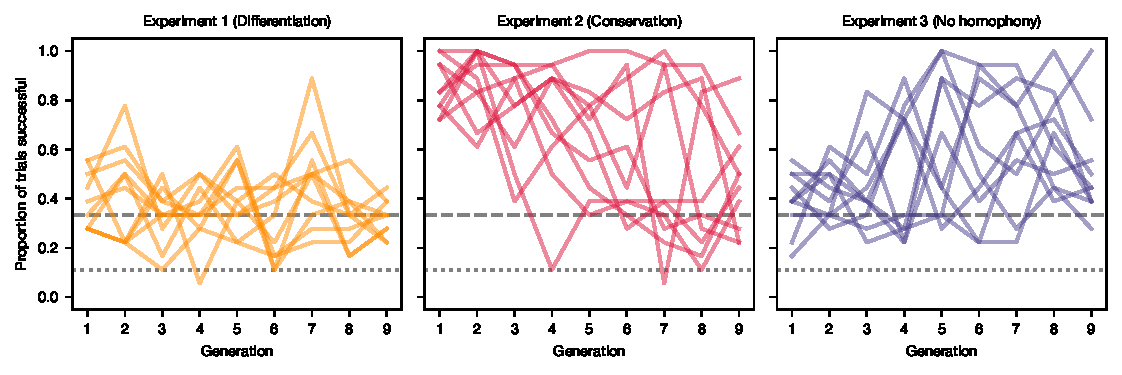
\includegraphics[scale=0.8]{figs/success.pdf}}
	\vspace*{2pt}
	\caption{Communicative success by generation in the communicative conditions of all three experiments. The dotted line shows chance level if the comprehending participant selects from the array of nine items at random (i.e., 1/9), and the dashed line shows chance level if the comprehending participant knows the correct shape but selects color at random (i.e., 1/3).}
	\label{success}
	\end{figure}

In general, it might be said that the maintenance of an optimal system is easier than the construction of a new one \parencite[see also][]{Smith:2002}. \newmaterial{This is made particularly salient by Fig.~\ref{success}, which compares the experiments in terms of communicative success (the proportion of trials in which the comprehending participant selected the correct target item in response to their partner). In Experiment~1, communicative success remains around chance level (a one in three probability of selecting the right color) because the orthographic systems tend to become uninformative, mirroring the spoken form of the language. In Experiment~2, by comparison, communicative success remains high in several of the chains (i.e., those chains that preserved the expressive system). This suggests that, while it may be difficult for participants to establish an informative writing system, it is comparatively easy to preserve an informative system that offers a clear advantage. It is also interesting to observe what happens to communicative success in Experiment~3 when the homophony pressure is removed. Here, communicative success \textit{does} increase over time, as the participants---unencumbered by having to represent sound---find communicative strategies to differentiate meaning. Taken together, these results suggest that it is difficult for the differentiation mechanism to operate in the face of homophony, but comparatively easy for the conservation mechanism to operate under these same circumstances.}

\subsection{Limitations}

These conclusions must be interpreted within the limitations of these experiments, which are, after all, highly simplified simulacra of real-world processes. Besides the general scaling-down of orthography, phonology, morphology, and semantics to an experimentally tractable test case, one notable issue we faced was how to induce pressure for informativeness in the written modality. We follow a large body of recent studies by using a real-time communication game \parencite[e.g.,][]{Carr:2017, Kanwal:2017, Kirby:2015, Raviv:2018, Saldana:2019, Silvey:2019, Winters:2015}, but such games are not very representative of the dynamics involved in asynchronous written communication \parencite[although see][for some approaches]{Winters:2019}. That being said, much written communication in the present day is indeed synchronous (e.g., text messaging), potentially allowing the dynamics typically associated with synchronous communication, such as feedback, to play a role in the development of written forms of the language \parencite{Lupyan:2016}.

Another limitation of this work is the extent to which lexical disambiguation really matters in real-world reading scenarios, since the syntactic and semantic context usually makes the meaning clear. If \textit{knight} and \textit{night} were spelled the same way, it is hard to imagine a context in which they might be confused. That being said, cultural transmission has been argued to have a strong amplifying effect on small cognitive biases \parencite{Thompson:2016}, so perhaps even a minor benefit in reading could have a large effect on orthography. An important issue in pursuit of this hypothesis will be to better understand the mechanism by which the biases of readers might place selective pressure on a writing system that is primarily shaped by the needs and preferences of writers, \newmaterial{especially given that writing systems are often fixed cultural fossils that do not readily adapt to external pressures.} It is also important to note that the functional explanation for heterography advanced here (i.e., ambiguity avoidance) is likely to be one of many. For example, \textcite{Stenroos:2016} take the view that English spelling has generally remained opaque with respect to phonology because its primary function was to be a record keeper across time and space. From this perspective, written forms of language resist change because they need to be accessible across decades or centuries and across different jurisdictions or dialect areas.

\newmaterial{The results of both experiments were relatively weak statistically, with the differences in terms of informativeness between the Transmission-only and Transmission~+ Communication conditions only just (or not quite) meeting the 95\% criterion. This is likely to be related to a combination of two factors: a relatively small effect size combined with a relatively small sample size, with only ten chains---ten independent sampling units---in each condition. This is a general issue with iterated learning experiments that results from their resource-intensive nature, and our use of ten chains follows or exceeds norms in the field \parencite[e.g.,][]{Kempe:2015, Kirby:2008, Kirby:2015, Raviv:2018, Roberts:2018, Smith:2010, Tamariz:2015}. Nevertheless, our study suggests that future work in this area could benefit from increased power.}

\newmaterial{One important thing to note is that the participant population we draw from (native English speakers) is already accustomed to heterography and opacity; informative orthography might be even less forthcoming in other populations used to more transparent writing systems. This brings us to a much deeper issue with iterated learning experiments in general: We cannot avoid the fact that our participants come into the lab with prior linguistic baggage, whether that baggage is for the encoding of sound or the encoding of meaning. Ideally, our experiments would be performed with participants who have no writing experience at all, but since that would be very difficult to achieve, perhaps the second-best option is a participant population that is relatively open-minded to both types of writing systems. In this sense, our use of English speakers is actually quite appropriate, since the English writing system is neither fully phonographic nor fully logographic.}

\section{Conclusion}

\newmaterial{It has long been known that heterography makes reading and learning to read difficult \parencite{Pexman:2001, Seymour:2003}. As a result, heterography has often been derided as a source of unnecessary complexity, and the orthographic reforms implemented in many languages have tended to focus on its elimination. However, recent research suggests that heterography may in some circumstances be functional because it permits rapid access to meaning \parencite{Rastle:2019, Ulicheva:2020}. The novel research presented in this article suggests that the cultural evolution of writing systems may prefer to trade some simplicity for greater informativeness when the communicative need for disambiguation is strong enough. These results imply that writing systems may, under some circumstances, evolve to fill a “reading niche.” However, our research also shows that creating heterography, and even maintaining it, is challenging given the demands it poses on learning. These findings raise the prospect of a third major issue relevant to the cultural evolution of writing systems: education. Instead of yielding to the pressure of learnability, orthographies like English and Chinese have developed and maintained a high degree of informativeness because those societies have invested in education systems that spend many years teaching children to read \parencite[e.g.,][]{Xinchun:1999}. Thus, informative writing systems that contribute to rapid, skilled reading may not only impose learning costs, but may also require ongoing economic investment.}

%~%~%~%~%~%~%~%~%~%~%~%~%~%~%~%~%~%~%~%~%~%~%~%~%~%~%~%~%~%~%~%~%~%~%~%~%~%~%~%~%~%~%~%~%~%~%~%~%~%~%~%

% \section{Acknowledgments}

% \noindent This work was funded by a Leverhulme Trust Research Project Grant (grant number: RPG-2020-034).

\printbibliography

%~%~%~%~%~%~%~%~%~%~%~%~%~%~%~%~%~%~%~%~%~%~%~%~%~%~%~%~%~%~%~%~%~%~%~%~%~%~%~%~%~%~%~%~%~%~%~%~%~%~%~%

\clearpage

\appendix

\section{Participant instructions}

\begin{figure}[h!]
\makebox[\textwidth][c]{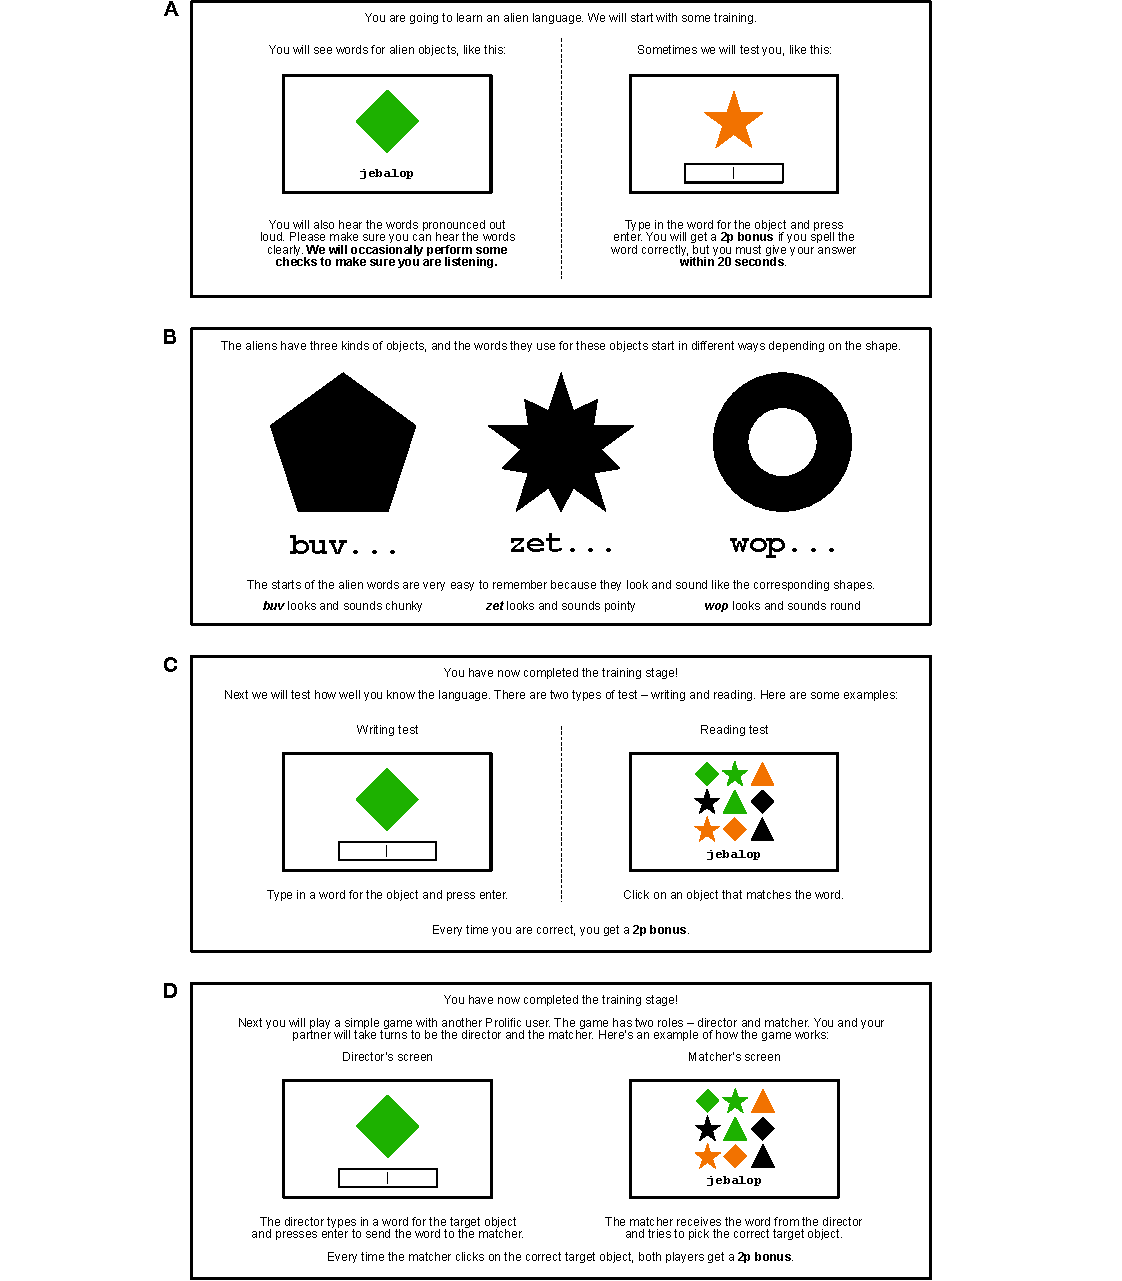
\includegraphics[scale=0.8]{figs/instructions.pdf}}
\vspace*{2pt}
\caption{\textbf{A} Training instructions. \textbf{B} Explicit prefix training. \textbf{C} Test instructions in the Transmission-only condition. \textbf{D} Communication game instructions in the Transmission + Communication condition (an animation, which can be viewed in the OSF repository, showed examples of successful and unsuccessful trials).}
\label{supp_training}
\end{figure}

\clearpage

\section{Posterior parameter estimates and diagnostics}

These tables provide detailed posterior parameter estimates for each of the three experiments, including the posterior differences between conditions. The means and standard deviations characterize the central tendency and width of the posterior. The 95\% HDI is the narrowest interval that includes 95\% of the posterior probability mass. The effective sample size (ESS) is the effective number of samples drawn from the posterior after accounting for autocorrelation in the MCMC chains; values above 10,000 are recommended for numerical stability. $\hat{R}$ is a measure of convergence across the independent MCMC chains used to sample from the posterior; values close to 1 indicate high convergence.

\begin{table}[h]
\begin{center}
\begin{threeparttable}
\caption{Experiment 1}
\footnotesize
\begin{tabular}{lrrrlrr}
\toprule
 & Mean & SD & \multicolumn{2}{c}{95\% HDI} & ESS & $\hat{R}$ \\
\midrule
\multicolumn{7}{c}{Probability informative} \\
$\alpha_\mathrm{trans}$ & 6.77 & 1.79 & 3.51 & 10.43 & 51930 & 1.00 \\
$\beta_\mathrm{trans}$ & -6.47 & 1.56 & -9.61 & -3.64 & 36904 & 1.00 \\
$\alpha_\mathrm{comm}$ & 2.23 & 0.76 & 0.78 & 3.74 & 65662 & 1.00 \\
$\beta_\mathrm{comm}$ & -1.94 & 0.55 & -3.05 & -0.91 & 34929 & 1.00 \\
$\Delta(\alpha)$ & -4.54 & 1.95 & -8.41 & -0.82 & 51523 & 1.00 \\
$\Delta(\beta)$ & 4.53 & 1.65 & 1.48 & 7.88 & 35250 & 1.00 \\
\midrule
\multicolumn{7}{c}{Communicative cost} \\
$\alpha_\mathrm{trans}$ & 0.14 & 0.08 & -0.03 & 0.30 & 68812 & 1.00 \\
$\beta_\mathrm{trans}$ & 0.60 & 0.07 & 0.47 & 0.73 & 30143 & 1.00 \\
$\alpha_\mathrm{comm}$ & 0.15 & 0.11 & -0.07 & 0.36 & 75737 & 1.00 \\
$\beta_\mathrm{comm}$ & 0.43 & 0.07 & 0.28 & 0.57 & 57053 & 1.00 \\
$\Delta(\alpha)$ & 0.01 & 0.14 & -0.26 & 0.28 & 74870 & 1.00 \\
$\Delta(\beta)$ & -0.17 & 0.10 & -0.36 & 0.02 & 40473 & 1.00 \\
\midrule
\multicolumn{7}{c}{Transmission error} \\
$\alpha_\mathrm{trans}$ & 0.94 & 0.08 & 0.77 & 1.11 & 105363 & 1.00 \\
$\beta_\mathrm{trans}$ & -0.39 & 0.05 & -0.48 & -0.29 & 101977 & 1.00 \\
$\alpha_\mathrm{comm}$ & 1.17 & 0.15 & 0.86 & 1.47 & 95553 & 1.00 \\
$\beta_\mathrm{comm}$ & -0.35 & 0.10 & -0.54 & -0.17 & 58199 & 1.00 \\
$\Delta(\alpha)$ & 0.23 & 0.18 & -0.12 & 0.57 & 98993 & 1.00 \\
$\Delta(\beta)$ & 0.03 & 0.11 & -0.18 & 0.24 & 64129 & 1.00 \\
\bottomrule
\end{tabular}
\label{exp1_parameter_estimates}
\end{threeparttable}
\end{center}
\end{table}

\begin{table}[h]
\begin{center}
\begin{threeparttable}
\caption{Experiment 2}
\footnotesize
\begin{tabular}{lrrrrrr}
\toprule
 & Mean & SD & \multicolumn{2}{c}{95\% HDI} & ESS & $\hat{R}$ \\
\midrule
\multicolumn{7}{c}{Probability informative} \\
$\alpha_\mathrm{trans}$ & 14.14 & 3.45 & 7.75 & 20.96 & 75580 & 1.00 \\
$\beta_\mathrm{trans}$ & -5.89 & 1.35 & -8.60 & -3.43 & 79605 & 1.00 \\
$\gamma_\mathrm{trans}$ & -0.22 & 0.68 & -1.57 & 1.14 & 67339 & 1.00 \\
$\alpha_\mathrm{comm}$ & 12.52 & 3.36 & 6.45 & 19.25 & 42630 & 1.00 \\
$\beta_\mathrm{comm}$ & -3.24 & 0.98 & -5.22 & -1.39 & 56677 & 1.00 \\
$\gamma_\mathrm{comm}$ & -0.98 & 0.64 & -2.25 & 0.28 & 70323 & 1.00 \\
$\Delta(\alpha)$ & -1.62 & 4.82 & -11.03 & 7.90 & 47446 & 1.00 \\
$\Delta(\beta)$ & 2.65 & 1.67 & -0.58 & 5.95 & 66432 & 1.00 \\
$\Delta(\gamma)$ & 4.91 & 1.49 & 2.13 & 7.92 & 75152 & 1.00 \\
\midrule
\multicolumn{7}{c}{Communicative cost} \\
$\alpha_\mathrm{trans}$ & -0.63 & 0.14 & -0.89 & -0.35 & 64515 & 1.00 \\
$\beta_\mathrm{trans}$ & 0.52 & 0.07 & 0.38 & 0.66 & 26030 & 1.00 \\
$\gamma_\mathrm{trans}$ & 0.09 & 0.04 & 0.02 & 0.16 & 98284 & 1.00 \\
$\alpha_\mathrm{comm}$ & -0.50 & 0.13 & -0.75 & -0.26 & 65698 & 1.00 \\
$\beta_\mathrm{comm}$ & 0.32 & 0.07 & 0.18 & 0.46 & 24609 & 1.00 \\
$\gamma_\mathrm{comm}$ & 0.10 & 0.04 & 0.02 & 0.18 & 89149 & 1.00 \\
$\Delta(\alpha)$ & 0.13 & 0.18 & -0.24 & 0.49 & 66441 & 1.00 \\
$\Delta(\beta)$ & -0.20 & 0.10 & -0.40 & -0.00 & 24592 & 1.00 \\
$\Delta(\gamma)$ & -0.42 & 0.08 & -0.57 & -0.25 & 31416 & 1.00 \\
\midrule
\multicolumn{7}{c}{Transmission error} \\
$\alpha_\mathrm{trans}$ & 0.18 & 0.16 & -0.14 & 0.50 & 133362 & 1.00 \\
$\beta_\mathrm{trans}$ & 0.11 & 0.06 & -0.00 & 0.23 & 101042 & 1.00 \\
$\gamma_\mathrm{trans}$ & -0.02 & 0.06 & -0.13 & 0.09 & 110157 & 1.00 \\
$\alpha_\mathrm{comm}$ & 0.10 & 0.18 & -0.25 & 0.44 & 87045 & 1.00 \\
$\beta_\mathrm{comm}$ & 0.16 & 0.06 & 0.05 & 0.28 & 95395 & 1.00 \\
$\gamma_\mathrm{comm}$ & -0.02 & 0.06 & -0.14 & 0.09 & 95801 & 1.00 \\
$\Delta(\alpha)$ & -0.08 & 0.24 & -0.55 & 0.39 & 110229 & 1.00 \\
$\Delta(\beta)$ & 0.05 & 0.08 & -0.12 & 0.21 & 97655 & 1.00 \\
$\Delta(\gamma)$ & -0.14 & 0.08 & -0.30 & 0.03 & 98052 & 1.00 \\
\bottomrule
\end{tabular}
\label{exp2_parameter_estimates}
\end{threeparttable}
\end{center}
\end{table}

\begin{table}[h]
\begin{center}
\begin{threeparttable}
\caption{Experiment 3 (compared to Exp. 1, Comm.)}
\footnotesize
\begin{tabular}{lrrrlrr}
\toprule
 & Mean & SD & \multicolumn{2}{c}{95\% HDI} & ESS & $\hat{R}$ \\
\midrule
\multicolumn{7}{c}{Probability informative} \\
$\alpha_\mathrm{exp1}$ & 2.23 & 0.76 & 0.78 & 3.74 & 65662 & 1.00 \\
$\beta_\mathrm{exp1}$ & -1.94 & 0.55 & -3.05 & -0.91 & 34929 & 1.00 \\
$\alpha_\mathrm{exp3}$ & 1.46 & 0.66 & 0.19 & 2.78 & 74546 & 1.00 \\
$\beta_\mathrm{exp3}$ & -0.25 & 0.38 & -1.02 & 0.49 & 73672 & 1.00 \\
$\Delta(\alpha)$ & -0.76 & 1.01 & -2.76 & 1.21 & 63934 & 1.00 \\
$\Delta(\beta)$ & 1.69 & 0.67 & 0.40 & 3.04 & 39662 & 1.00 \\
\midrule
\multicolumn{7}{c}{Communicative cost} \\
$\alpha_\mathrm{exp1}$ & 0.15 & 0.11 & -0.07 & 0.36 & 75737 & 1.00 \\
$\beta_\mathrm{exp1}$ & 0.43 & 0.07 & 0.28 & 0.57 & 57053 & 1.00 \\
$\alpha_\mathrm{exp3}$ & 0.36 & 0.13 & 0.12 & 0.61 & 101323 & 1.00 \\
$\beta_\mathrm{exp3}$ & 0.10 & 0.08 & -0.06 & 0.25 & 72628 & 1.00 \\
$\Delta(\alpha)$ & 0.21 & 0.17 & -0.11 & 0.54 & 89412 & 1.00 \\
$\Delta(\beta)$ & -0.33 & 0.11 & -0.54 & -0.12 & 62222 & 1.00 \\
\midrule
\multicolumn{7}{c}{Transmission error} \\
$\alpha_\mathrm{exp1}$ & 1.17 & 0.15 & 0.86 & 1.47 & 95553 & 1.00 \\
$\beta_\mathrm{exp1}$ & -0.35 & 0.10 & -0.54 & -0.17 & 58199 & 1.00 \\
$\alpha_\mathrm{exp3}$ & 1.35 & 0.20 & 0.97 & 1.75 & 82673 & 1.00 \\
$\beta_\mathrm{exp3}$ & -0.28 & 0.12 & -0.50 & -0.05 & 75632 & 1.00 \\
$\Delta(\alpha)$ & 0.19 & 0.25 & -0.30 & 0.69 & 87400 & 1.00 \\
$\Delta(\beta)$ & 0.08 & 0.15 & -0.22 & 0.37 & 66566 & 1.00 \\
\bottomrule
\end{tabular}
\label{exp3_parameter_estimates}
\end{threeparttable}
\end{center}
\end{table}

\clearpage

\section{Experiment 3}

Our Experiment~1 results were surprising in that they failed to find much evidence for the emergence of clear, systematic, informative systems, even under communicative pressure with financial incentive. One possible concern put forward during review was that there might be some other spurious reason why participants failed to differentiate the spellings in the communicative condition. The Experiment~1 finding might perhaps have been explained by participants not understanding the communicative goal of the study or some other subtle methodological issue. Our position was that the lack of differentiation was due to the very strong homophony pressure; participants found it difficult to learn, create, and produce spellings that contradicted the spoken form. To test whether the lack of informativeness might be attributed to the homophony pressure and to check that the communicative pressure was, in~principle, sufficient to promote more informative systems, we ran a third experiment that entirely removed the spoken modality.

\subsection{Methods}

The methods were identical to the Transmission~+ Communication condition of Experiment~1 with two exceptions. First, no spoken forms were provided to participants during training or test. This removes any homophony pressure and brings the experimental design into alignment with most prior studies, which are generally only orthographic in nature \parencite[e.g.,][]{Kirby:2008, Kirby:2015, Beckner:2017}. Second, a new set of spellings was selected to initialize the chains. This was because our goal was to remove all traces of homophony but the Experiment~1 seed spellings (<coh>, <koe>, <co>, etc.) were likely to be perceived as homophonous, even if they were not explicitly given any phonological value.

\subsubsection{Participants}

The experiment was completed by 230 native-English participants, who were recruited through Prolific and paid £2.50 for participation. The median bonus was £0.70 and the median completion time was 17~m, resulting in a median hourly rate of £8.78 (£11.08 including bonus). 26 participants were excluded because they (or their partners) used English color words, and a further 24 participants were lost to communication-game pairing failures. The final dataset comprises 180 participants (10 chains of 9 pairs of participants).

\subsubsection{Stimuli}

The suffixes used to initialize the chains consisted of a consonant grapheme from the set \{<k>, <m>, <s>\} concatenated with a vowel grapheme from the set \{<a>, <ei>, <oe>\}. The nine resulting suffixes were mapped to the nine possible objects randomly (without replacement). This procedure was identical to Experiment~1, except for the change in grapheme identities, which were chosen because their conventional phonological values are very different from each other (i.e., different places and manners of articulation).

\subsection{Results}

	\begin{figure}
	\makebox[\textwidth][c]{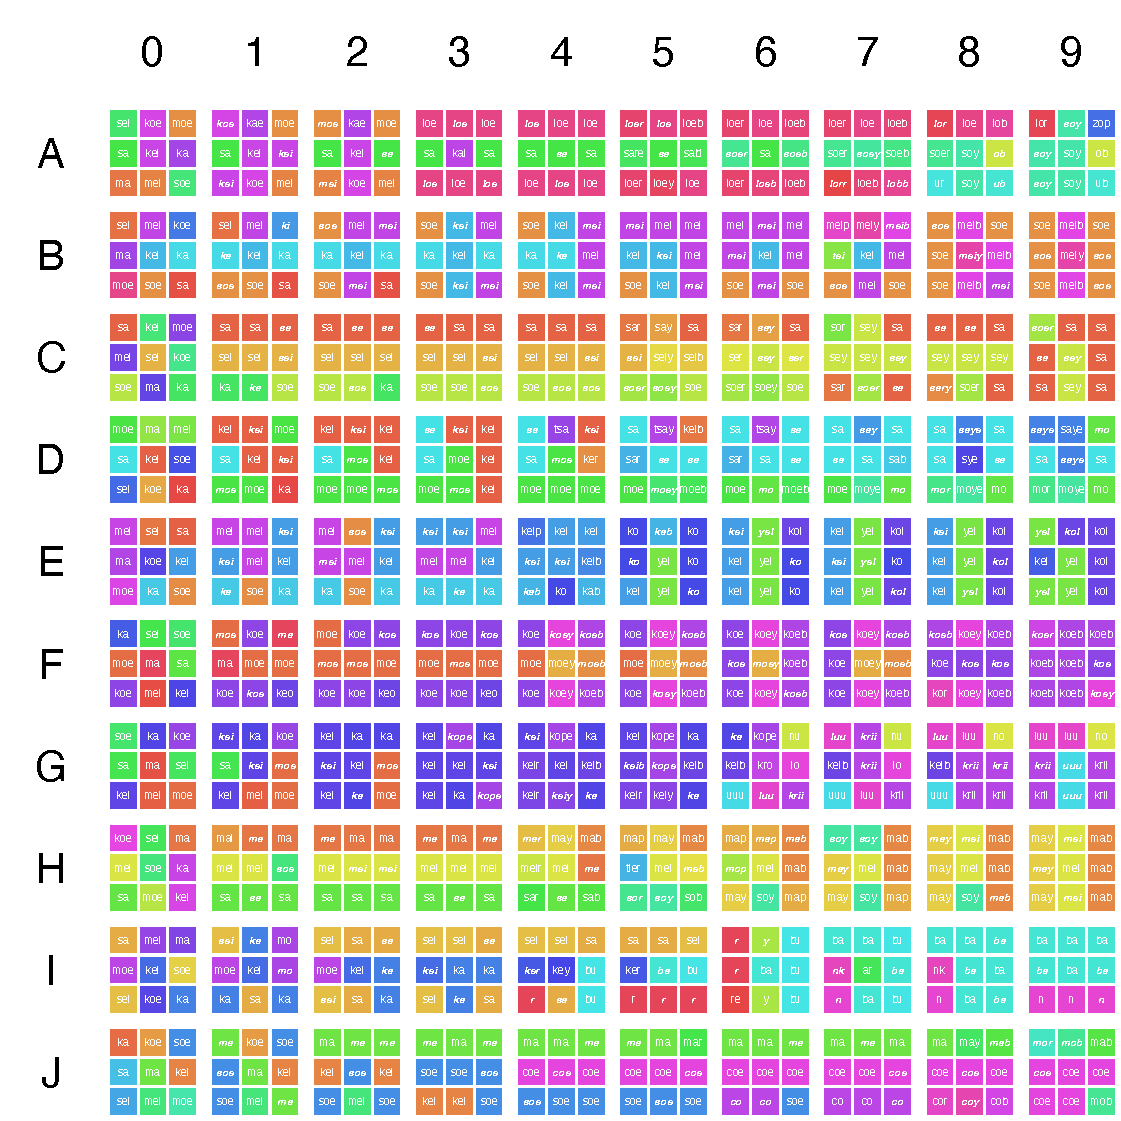
\includegraphics[scale=0.8]{figs/sil_com.pdf}}
	\vspace*{2pt}
	\caption{Results from Experiment~3. Each matrix shows the suffix spelling system in use at a particular generation (shape on the rows, color on the columns). Chains are labeled A--J and generations are labeled 0–9 (0 is the randomly generated seed system). Each chain uses an independent color palette, with each color representing a particular suffix spelling; similar colors indicate similar spellings. Spellings in bold-italic are the generalizations on unseen items.}
	\label{sil_com}
	\end{figure}

Fig.~\ref{sil_com} plots all suffix spellings by chain and generation. The most notable difference in comparison to Experiment~1 was the large number of times participants used English to signal color. Like the main experiments, we rejected participants who used full color words. The proportion of participants rejected for this reason was almost four times higher (10.4\% in Experiment~3 vs.\@ 2.8\% in Experiment~1). In addition, participants were much more likely to append English color letters: All ten chains converged on this solution, typically around Generation~4 or~5. In comparison, only five of the chains in Experiment~1 adopted this solution. In the absence of any spoken form and in the absence of any explicit instruction not to use English, participants appear to find the use of English to be the simplest strategy for marking color. Importantly, the widespread use of English suggests that participants did indeed understand the communicative need to mark color.

	\begin{figure}
	\makebox[\textwidth][c]{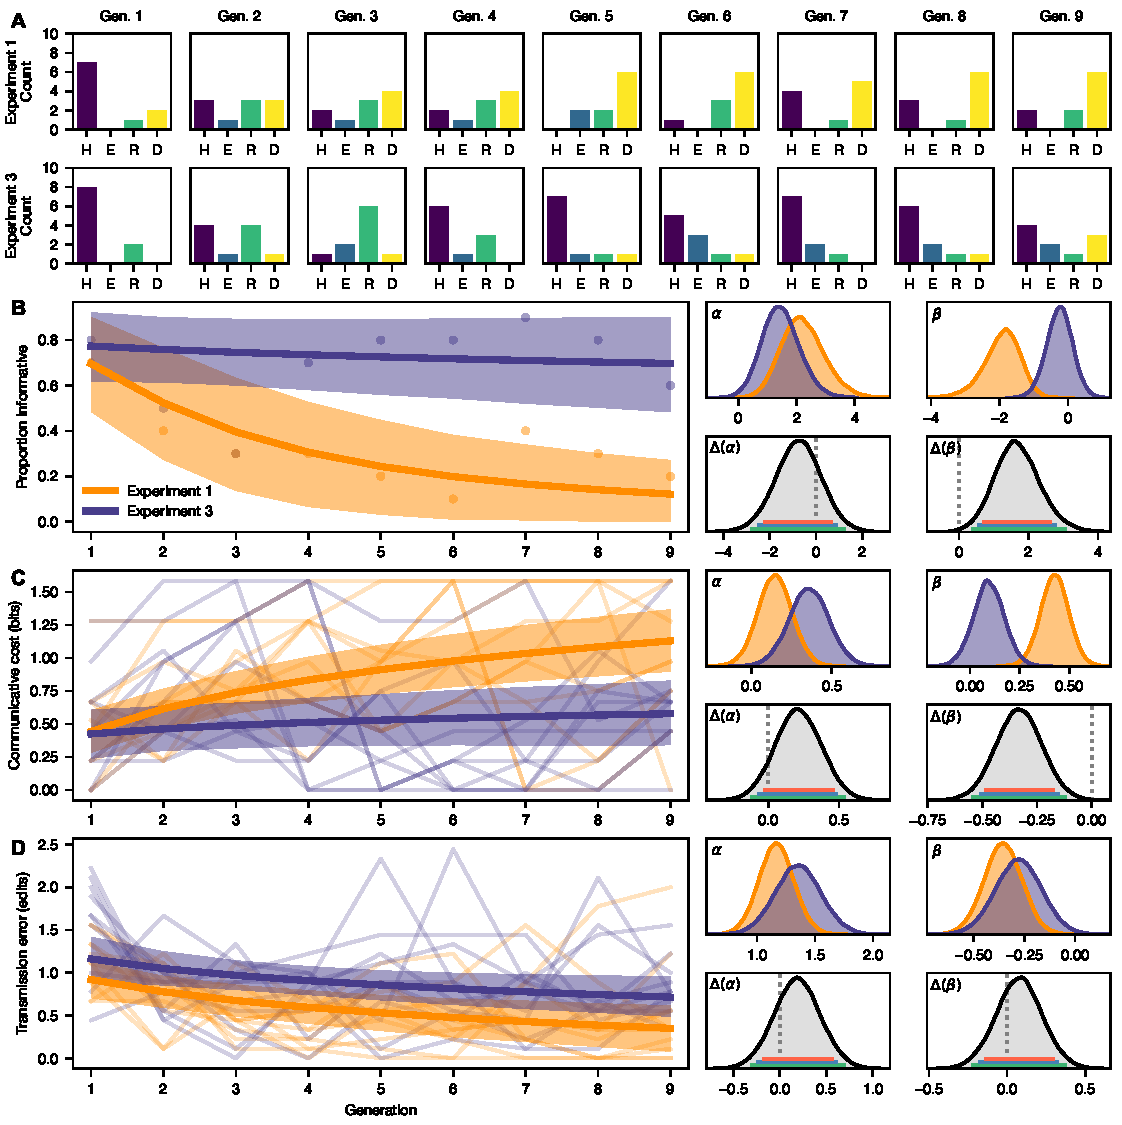
\includegraphics[scale=0.8]{figs/results_exp3.pdf}}
	\vspace*{2pt}
	\caption{Results of Experiment~3. \textbf{A} Typological distribution by generation and condition over the four typological categories: holistic (H; purple), expressive (E; blue), redundant (R, green), and degenerate (D; yellow). \textbf{B} Proportion of systems classified as informative (holistic or expressive) by generation. The dots show the observed proportions and the curves show logistic regression models fit to the data. \textbf{C} Communicative cost by generation along with regression models fit to the data. \textbf{D} Transmission error by generation along with regression models fit to the data. The panels on the right show the posterior estimates of the intercept ($\alpha$) and slope ($\beta$) parameters by condition as well as the posterior differences between conditions. The green, blue, and red bars indicate respectively the 95\%, 90\%, and 85\% HDIs (credible intervals).}
	\label{results_exp3}
	\end{figure}

Aside from the use of English, there were also some instances of expressive systems emerging, notably E8 (<kei>, <yel>, <kol>) and H9 (<may>, <mei>, <mab>), but also B4, D3, E2 (semi-expressive systems). In addition, many of the cases of English color marking mentioned above can be analyzed as expressive systems if you reconsider which part of the word is the stem. For example, the system that emerged in Chain~F seems to treat the stems as <buvikoe->, <zetimoe->, <wopikoe-> and the suffixes as $\emptyset$ (pink), <-y> (yellow), <-b> (blue).

The quantitative results are plotted in Fig.~\ref{results_exp3} and are compared against the equivalent results from Experiment~1 (the Transmission~+ Communication condition). Overall, the effect of removing the homophony pressure was to prevent the systems from degenerating over time---both measures of informativeness show a clear difference in slopes, and informativeness levels remain fairly constant over time in Experiment~3, mainly in the form of holistic systems.

\subsection{Summary}

Our first aim with Experiment~3 was to perform an additional check on whether participants understood the nature of the communicative task. By removing the homophony, Experiment~3 becomes equivalent to prior iterated learning studies, meaning that we should have been able to replicate the finding that informativeness remains high under communicative need. The results showed that participants were much more willing to innovate and differentiate when unconstrained by the presence of spoken forms. In particular, the widespread use of English as a strategy for marking color suggests that participants did indeed understand the need for disambiguation and were willing to diverge from their training material if it seemed advantageous to do so. Our second aim with Experiment~3 was to better understand whether the presence of homophonous spoken forms in Experiment~1 prevented the emergence of informative orthographic systems. The results suggested that this is indeed the case: The systems tended not to degenerate in Experiment~3 and instead tended to remain informative usually by adopting some form of English-based suffixes.

Like Experiment~1, however, there was still a notable lack of expressive systems in Experiment~3. Why might this be the case? One possibility is that there was insufficient simplicity pressure to produce expressive systems (both in this experiment and the main experiments). Recall that the holistic and expressive systems are both informative about color; the expressive system is just a simpler way of marking color. With this in mind, expressive systems require not only sufficient pressure for informativeness (induced through the communicative task), but also sufficient pressure for simplicity (induced through learning). Given the small scale of our stimulus space---just nine items---it is perhaps the case that the simplicity pressure is not strong enough to give rise to the expressive solution; participants can achieve satisfactory performance without it. Consider also that, although expressive systems will be advantageous in the long run---making learning and communication easier for future generations of participant---it may not be particularly advantageous for the pair of participants at a given generation to radically alter the system; it may instead be more expedient to simply append English-based color markers onto the preexisting forms.

\end{document}